%--Metodologia

\section{MARCO DE REFERENCIA GENERAL}

%------------------------
\subsection{El COVID-19 en EE.UU.}

Según lo confirman los datos macros del impacto en la salud a causa de la pandemia, hasta el 08 de mayo del 2020, la crisis del COVID-19 a nivel global, confirmaba 3,755,220 casos, el fallecimiento de 265,187 personas, 1,200,503 recuperados y las pruebas o test realizadas a más de 36,567,435 ciudadanos en diversos países, para una población mundial estimada de 7,631,091,000 habitantes; de tales cifras se desprendía que el país Norteamericano continuaba siendo protagonista y epicentro de la epidemia con 1,066,564 casos confirmados  y  55,085 muertes según cifras del sitio Web: covid19datahub.io \footnote{\href{https://covid19datahub.io/}{https://covid19datahub.io/}}. Tal distribución de la concentración de las personas infectadas, se puede observar en el mapa de la Figura No.\eqref{fig:1}; conformado por 3,192 condados y ciudades, en el caso de Ilinois en la ciudad de Cook ya sobrepasaba a la ciudad de Nassau de New York con 50,236 casos y 2,197 muertes con una población de más de 5 millones de habitantes y una tasa de mortalidad de $0.04 \textperthousand$, las ciudades de Nassau y Suffolk del Estado de New York registraban 37,812 y 36,223 casos de covid-19 respectivamente y un total de 1,918 muertes para Nassau y 1,568 muertes para Suffolk; teniendo Nassau la tasa de mortalidad más alta de ambas ciudades con un $0.14 \textperthousand$.

\begin{figure}[H]
	\centering
	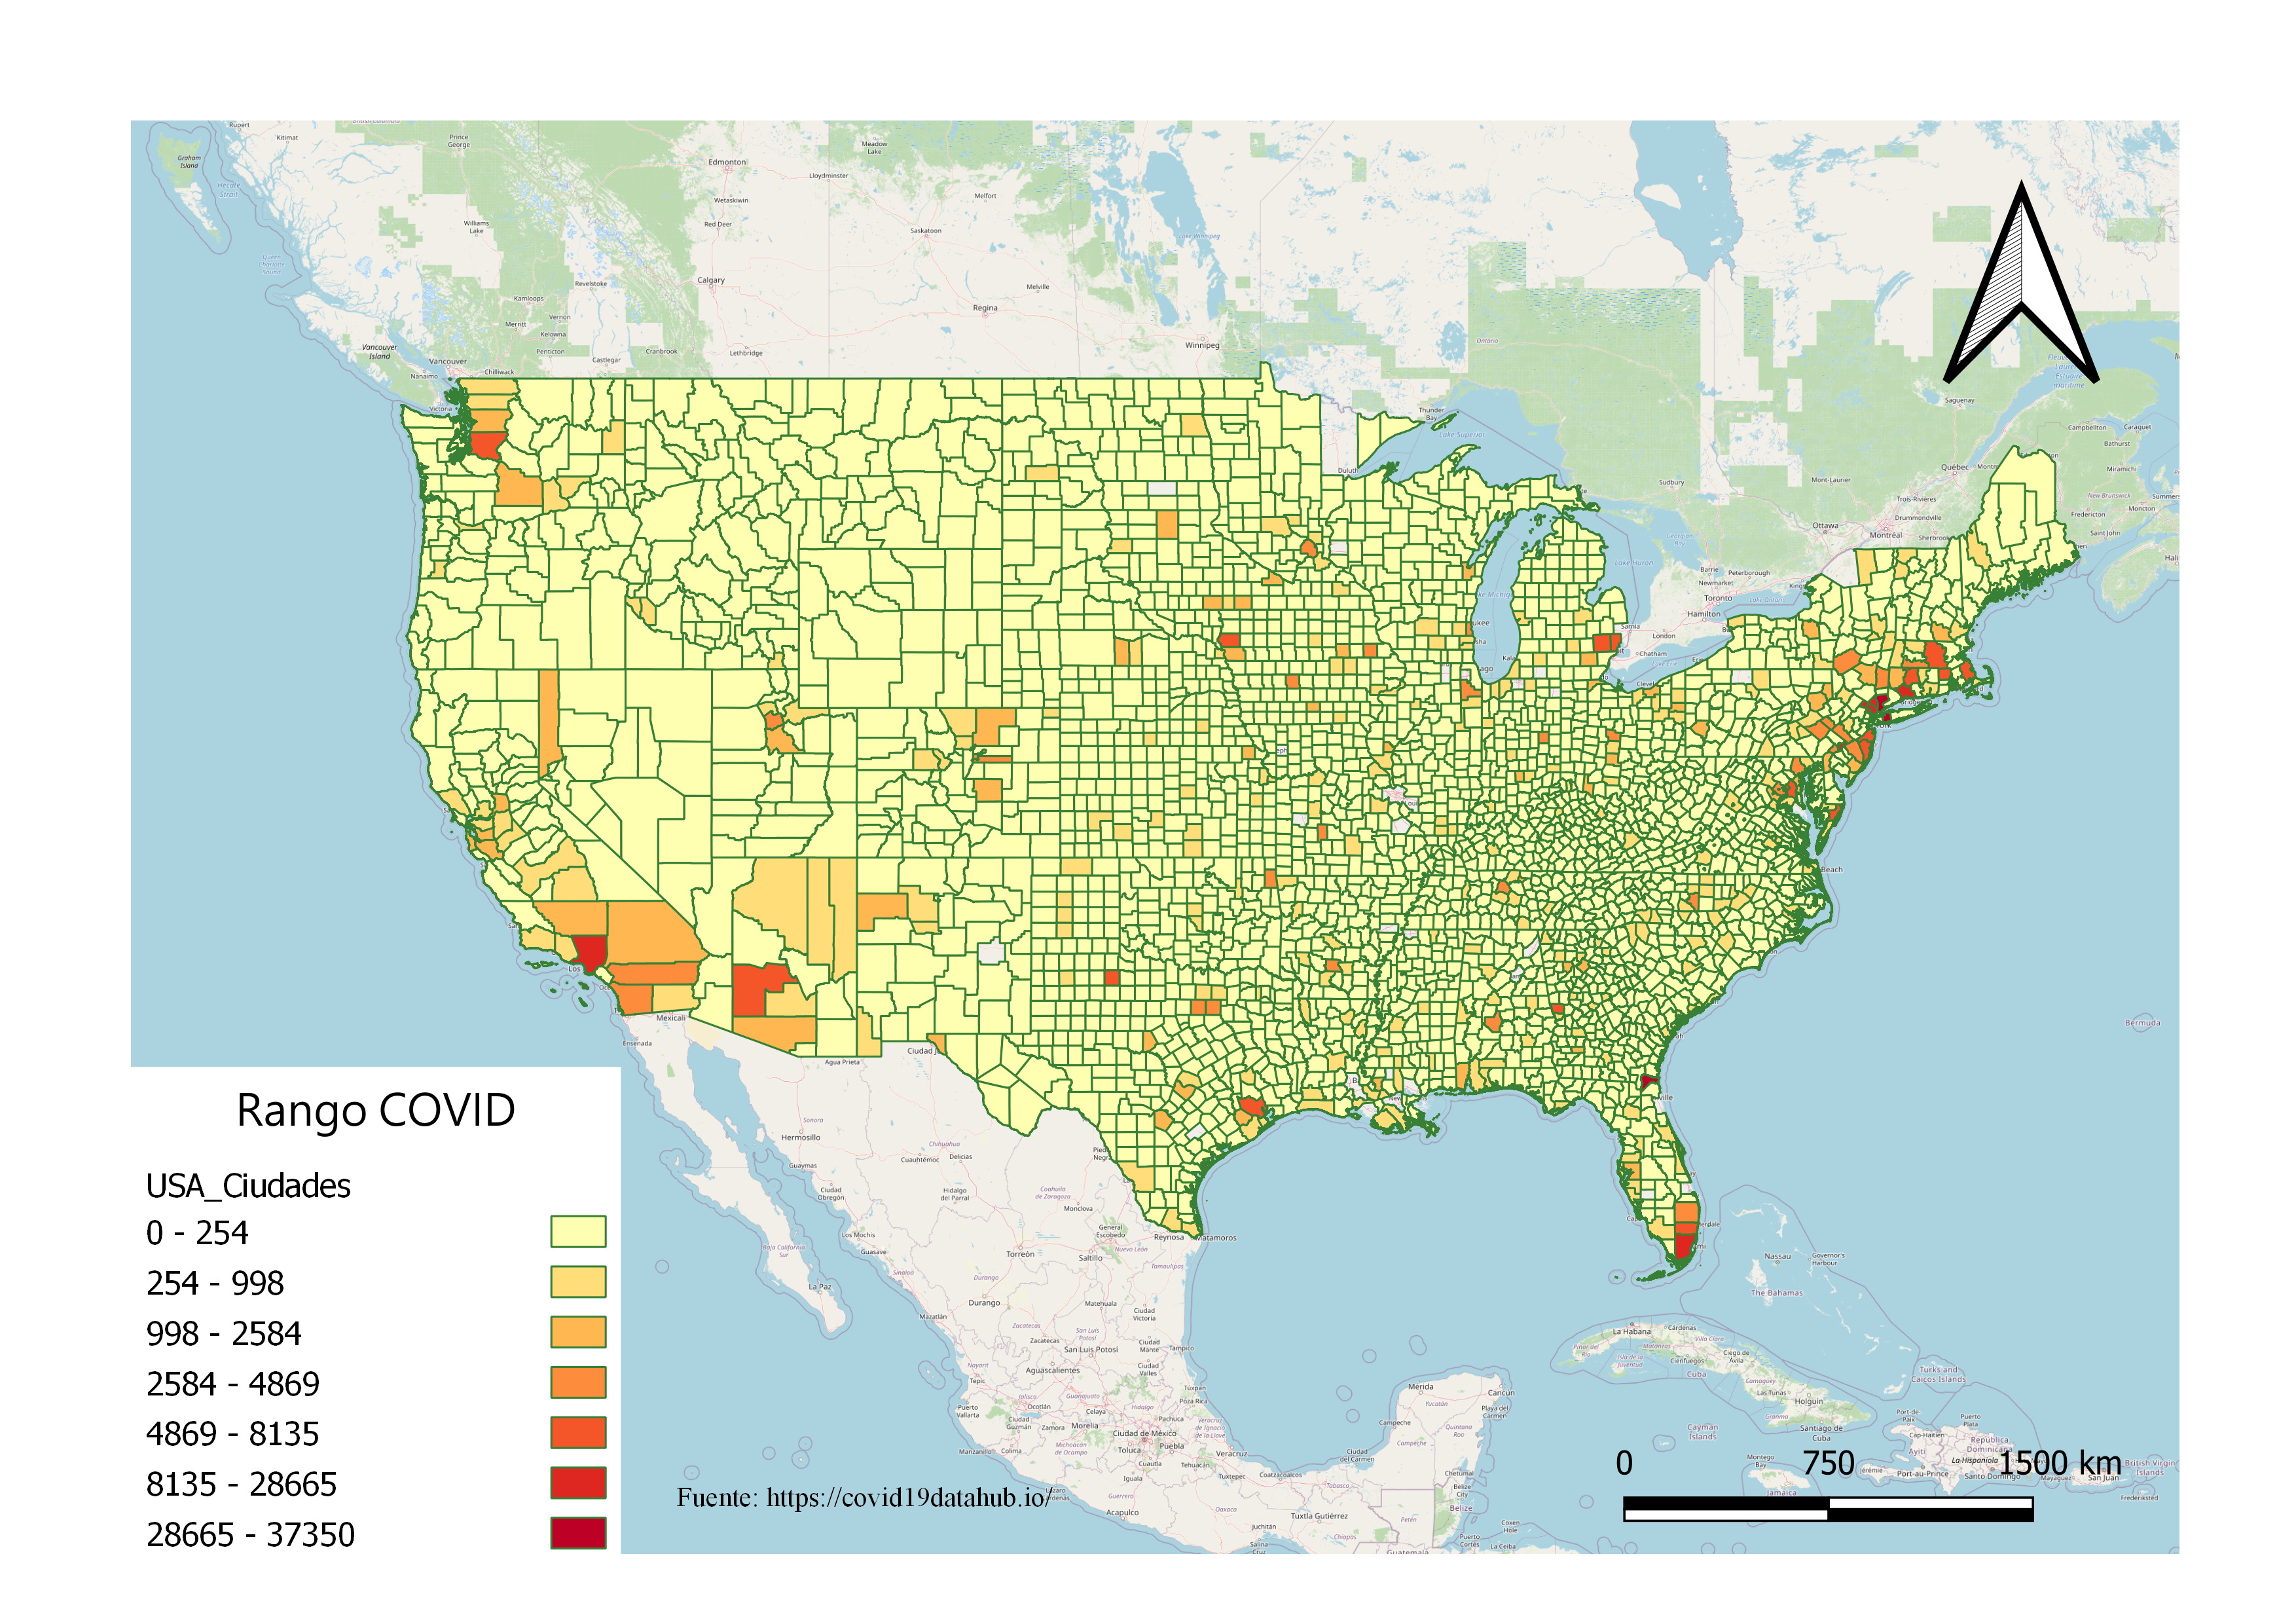
\includegraphics[width=1\linewidth]{Imagenes/MapaUSA2}
	\caption{\textbf{\textit{Mapa de los Estados Unidos que muestra la concentración de infectados del COVID-19, por ciudades y condados según rangos de casos confirmados.}} {\small El mapa de calor muestra los casos confirmados de covid-19 por cada uno de los 3,192 condados y ciudades del país, el ala este y suroeste de EE.UU. se observan con mayores focos de concentración del virus. Fuente: Elaboración propia con información de \href{https://covid19datahub.io/}{https://covid19datahub.io/}}
	} 
	\label{fig:1}
	\resizebox{20 cm}{!} { }
	
\end{figure}

A nivel geográfico por Estados, New York encaminaba la lista con más de 21,045 muertes, y 330,047 confirmados con una tasa de mortalidad por $0.09 \textperthousand$ para una población de 23,628,065 de ciudadanos, seguido de New Jersey con 135,454 casos confirmados, 8,952 fallecidos y una tasa de mortalidad de $0.10 \textperthousand$ con más de 8,882,190 habitantes, que junto a Massachusetts, Ilinois y California concentraban el $62 \textperthousand$ de todos los casos de población infectada por Coronavirus de los Estados Unidos, el detalle se puede observar en la Tabla No.\eqref{Tabla 1}; prácticamente toda el ala Este y Suroeste del país concentraban los mayores focos de infección de la pandemia al 08 de mayo.\\

Revisando la afectación por Estado es importante, según datos de la U.S. Census Bureau, Current Population Survey, Annual Social and Economic Supplement, 2018 \footnote{\href{https://www.census.gov/data.html}{https://www.census.gov/data.html}}; la población hispana se registraba en 59,763631 habitantes de los cuales un $9.3 \textperthousand$ eran centroamericanos y más del $62.3 \textperthousand$ eran mexicanos, dislumbrando no solo un problema de salud sino también económico; aquellos Estados que concentran más del $71.2 \textperthousand$ de población hispana son: California, Texas, Florida, New York, Arizona, Illinois y New Jersey con un total de 42,538,530 de residentes, mostrando gran parte de ellos una fuerte afectación por la epidemia del Covid-19.  

  \begin{table}[H]
	\centering
	\caption{\textbf{Principales Estados afectados por COVID-19, según población total e hispana}}
	\label{Tabla 1}
	\resizebox{17cm}{!} { 
		\begin{tabular}{lcccccc} \toprule			
			\textbf{Estado}	&	\textbf{Confirmados}	&	\textbf{Muertes}	&	\textbf{Población}	&	\textbf{Tasa de Muerte}	&	\textbf{Población Latina}	&	\textbf{Porcentaje Latino}	\\  \midrule
			New York	&	330,407	&	21,045	&	23,628,065	&	0.09	&	3,752,523	&	15.88	\\ 
			New Jersey	&	135,454	&	8,952	&	8,882,190	&	0.10	&	1,839,359	&	20.71	\\ 
			Massachusetts	&	75,333	&	4,702	&	6,892,503	&	0.07	&	846,780	&	12.29	\\ 
			Illinois	&	73,760	&	3,241	&	12,671,821	&	0.03	&	2,208,868	&	17.43	\\ 
			California	&	62,512	&	2,585	&	39,512,223	&	0.01	&	15,540,142	&	39.33	\\ 
			Pennsylvania	&	54,238	&	3,616	&	12,801,989	&	0.03	&	974,763	&	7.61	\\ 
			Michigan	&	46,326	&	4,393	&	9,986,857	&	0.04	&	517,381	&	5.18	\\ 
			Florida	&	39,199	&	1,738	&	21,477,737	&	0.01	&	5,562,452	&	25.90	\\ 
			Texas	&	36,609	&	1,004	&	28,995,881	&	0.00	&	11,368,844	&	39.21	\\ 
			Connecticut	&	32,411	&	2,874	&	3,565,287	&	0.08	&	589,810	&	16.54	\\ 
			Georgia	&	32,106	&	1,377	&	10,617,423	&	0.01	&	1,021,754	&	9.62	\\ 
			Louisiana	&	30,855	&	2,227	&	4,648,794	&	0.05	&	239,954	&	5.16	\\ 
			Maryland	&	30,485	&	1,560	&	6,045,680	&	0.03	&	628,435	&	10.39	\\ 
			&		&		&		&		&		&		\\ 
			\textbf{USA Total}	&	\textbf{1,091,514}	&	\textbf{56,645}	&	\textbf{326,610,817}	& \textbf{0.02}		&	\textbf{59,763,631}	& \textbf{18.30}		\\  \bottomrule
		

			
		\end{tabular} 
	
	}
	{\small \text{Fuente:Elaboración propia conforme a datos de U.S. Census Bureau y covid19datahub.io}}
	
\end{table}

Tal como lo muestra la Tabla No. 1, existe un alto riesgo que la crisis del Covid-19 cause problemas no solo en las condiciones de salud de la población hispana, sino que al verse afectada por las acciones de encierro dictadas por la cuarentena, puedan sufrir pérdida de sus empleos o una drástica reducción de ingresos, lo que puede traer a consecuencia una baja importante en la cuantía de transferencia en las remesas; el Banco Mundial proyecta que dicha reducción puede alcanzar US$\$ 445,000$ millones, es decir, un $19.7 \textperthousand$\footnote{\href{https://www.bancomundial.org/es/news/press-release/2020/04/22/world-bank-predicts-sharpest-decline-of-remittances-in-recent-history}{https://www.bancomundial.org/es/news/press-release/2020/04/22/world-bank-predicts-sharpest-decline-of-remittances-in-recent-history}}; el Estado de California muestra un nivel de comunidad hispana a un $39.33 \textperthousand$, Texas registra el $39.21 \textperthousand$ y New Jersey registra un $20.71 \textperthousand$ de habitantes hispanos, convirtiéndose en los estados que mayoritariamente concentra comunidad centroamericana y mexicana  y presentan un mejor nivel de empleos latinos en USA; Florida presenta un  $25.90 \textperthousand$, pero mayormente esta comunidad la conforma población Cubana.\\
 
%------------------ 
\subsection{Proyecciones de los Principales Indicadores Económicos de EE.UU. y el Mundo}

Intrínseco a la lucha contra el Covid-19 se encuentra la lucha por la economía, las proyecciones a nivel mundial acerca del impacto y crecimiento de las economías según los organismos internacionales, como el Fondo Monetario Internacional [FMI] \footnote{\href{https://www.imf.org/es/Publications/WEO/Issues/2020/04/14/weo-april-2020}{https://www.imf.org/es/Publications/WEO/Issues/2020/04/14/weo-april-2020}}, Banco Mundial [BM] \cite{mundial2020economia}, Comisión Económica para América Latina y El Caribe \cite{cepal2020dimensionar} y Banco Centroamericano de Integración Económica [BCIE] \cite{penafiel2020pandemia}, son diversas y hasta se cree bastantes modestas; tales proyecciones se resumen en la siguiente Tabla No. \eqref{Tabla 2}

  \begin{table}[H]
	\centering
	\caption{\textbf{Principales proyecciones económicas mundiales según organismos internacionales}}
	\label{Tabla 2}
	\resizebox{16cm}{!} { 
		\begin{tabular}{lccccccc} \toprule			
		\textbf{	Mundo/países/región}	&	\textbf{FMI 2020}	&	\textbf{FMI 2021}	&	\textbf{BM 2020}	&	\textbf{BM 2021}	&	\textbf{CEPAL 2020}	&	\textbf{BCIE 2020}	\\  \midrule
			Producto Mundial	&	-3.0	&	5.8	&	-3.0	&	5.8	&	-2.0	&	-4.7	\\ 
			Estados Unidos	&	\textbf{-5.9}	&	\textbf{4.7}	&	\textbf{-6.1}	&	\textbf{4.5}	&	\textbf{-3.8}	&	\textbf{-8.4}	\\ 
			Zona Euro	&	-7.5	&	4.7	&	-7.5	&	4.7	&	-5.7	&	-4.7	\\ 
			China	&	1.2	&	9.2	&	1.2	&	9.2	&	1.8	&	-9.7	\\  \bottomrule
				
			
		\end{tabular} 
		
	}
	{\small \text{Fuente:Elaboración propia conforme a datos de FMI,BM,CEPAL y BCIE (Escenarios Mckinsey)}}
	
\end{table}

Tanto el FMI y el BM proyectan para EE.UU. una caída no menor al $5 \textperthousand$, incluso la mayor caída la pronostica el BM con el $-6.1 \textperthousand$ y a través de los escenarios de Mckinsey presentados por el BCIE esta contracción llegaría a los $-8.4 \textperthousand$, lo que sería muy sensible para los intereses o expectativas económicas más optimistas y que proyectan un mejor cierre de la economía al final del año 2020, sin embargo, especialistas de la Reserva Federal, a través de un estudio proyectan que USA puede presentar impactos muy serios medidos en tres escenarios, según sea la perdida de capital:$-25 \textperthousand$,$-15 \textperthousand$ y $-5 \textperthousand$, \cite{kozlowski2020scarring} Julian Kozlowski, Laura Veldkamp y Venky Venkateswaran en su paper escrito en abril del presente año estiman tres escenarios por medio de un modelo econométrico para EE.UU.\footnote{\href{https://s3.amazonaws.com/real.stlouisfed.org/wp/2020/2020-009.pdf}{https://s3.amazonaws.com/real.stlouisfed.org/wp/2020/2020-009.pdf}}, observar Figura No \eqref{fig:2}:


\begin{figure}[H]
	\centering
	\resizebox{16 cm}{!} { 	
	\includegraphics[width=1\linewidth]{Imagenes/EscenariosUsa}}
	\caption{\textbf{\textit{Escenarios construidos para estimar el impacto en la economía de EE.UU. para el segundo trimestre.}} {\small El modelo econométrico consistía en resolver dos aspectos claves en primer lugar, debería medir los choques de productividad transitoria y depreciación de capital u obsolescencia que se usarían para describir el evento covid y en segundo lugar encontrar el ingrediente es un entorno donde la actividad económica es sensible a la probabilidad de choques extremos a los retornos de capital o la quiebra costosa, construido para tres escenarios de perdidas de capital: $-25 \textperthousand$,$-15 \textperthousand$ y $-5 \textperthousand$, para corto y largo plazo, Fuente:  \href{https://s3.amazonaws.com/real.stlouisfed.org/wp/2020/2020-009.pdf}{https://s3.amazonaws.com/real.stlouisfed.org/wp/2020/2020-009.pdf}}
	} 
	\label{fig:2}

	
\end{figure}	
	
En resumen en la Figura \eqref{fig:3} el escenario por perdida de capital por el $-25 \textperthousand$, para el segundo trimestre 2Q, podría ocasionar una contracción económica de hasta el $-18 \textperthousand$, estimación que será empleada en nuestro modelo para estimar la cuantía de las remesas. Pero estos insumos serán importantes, para el análisis, sin embargo observemos la tendencia actual de los principales indicadores macroeconómicos de una forma muy breve.

%-------------
\subsection{PIB y Desempleo en EE.UU.}

El PIB real de los EE.UU. para el primer trimestre mostró una contracción del $-1.2 \textperthousand$, tal como se observa en la Figura No.\eqref{fig:3}, ocasionado por el lockdown de muchos sectores estratégicos de la economía, pasando de US$\$ 19,221$ a US$\$ 18,987$ millones, las industrias o sectores que presentaron las mayores pérdidas fueron los sectores cárnicos, automovilístico, servicios por el lado de restaurantes, bares, hoteles, educación privada, tiendas departamentales, entre otras, industrias que han despedido parte o toda su fuerza de trabajo.    

\begin{figure}[H]
	\centering
	\resizebox{16.5cm}{!} { 
	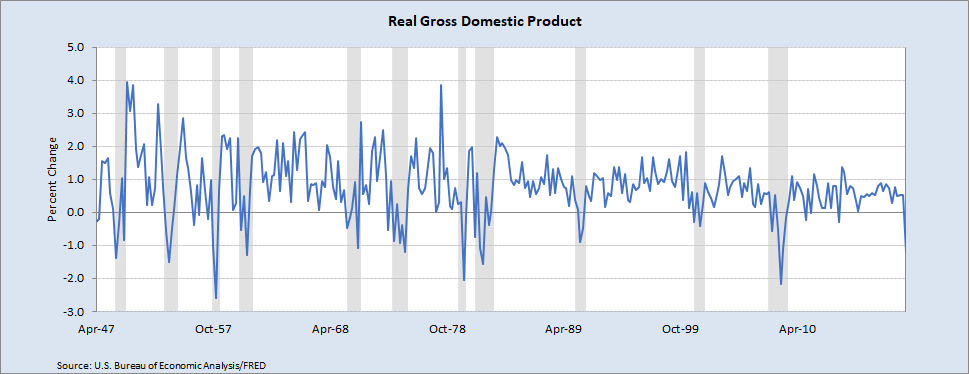
\includegraphics[width=1\linewidth]{Imagenes/PIB_USA}}
	\caption{\textbf{\textit{Tendencia del PIB Real trimestral de los EE.UU.}} {\small La tendencia se muestra hacia la baja y con pronostico de mayor contracción asociada a la cuarentena por el covid-19 que ha obligado a cerrar varias industrias, impactando también en el empleo. Fuente:  \href{https://www.govinfo.gov/app/collection/econi/2020/03/7}{https://www.govinfo.gov/app/collection/econi/2020/03/7}}
	} 
	\label{fig:3}
	
\end{figure}

Según las estadísticas del US Bureau of Labor Statistics\footnote{\href{https://www.bls.gov/news.release/empsit.t01.htm}{https://www.bls.gov/news.release/empsit.t01.htm}}, el desempleo para el mes de abril alcanzo los
$14.7 \textperthousand$, tal como lo muestra la Figura No. \eqref{fig:4}, el más alto de su historia, por arriba de las 11 recesiones económicas desde $1930$, con un total de 23 millones de desempleados para el mes de abril $2020$, el cual podría rondar los $30.2 $ millones acumulados, cifra realmente histórica, dicho desempleo afectó en mayor parte al empleo joven de entre los $ 16 - 19 $ años con un tasa registrada de $31.9 \textperthousand$ esto podría indicar problemas para aquellas personas que posean créditos de estudio y que su condición era trabajar y prepararse academicamente; de dicho desempleo las mujeres han sido las mayormente afectadas con una tasa de $15.5 \textperthousand$. y que se encuentran en edades de $20$ años o por arriba de ella. Los sectores con mayor impacto en el desempleo son Ocio y hospitalidad, que son servicios de hoteles, con el $39.3 \textperthousand$, con $4.8$ millones desocupados, Otros servicios registra $23.0 \textperthousand$ lo que representa $1.4$ millones de desempleados; Comercio mayorista y minorista reporta  $17.1 \textperthousand$, significando $3.2$ millones fuera del mercado laboral y finalmente el sector construcción en donde se emplean bastantes latinos pierde $1.5$ millones de trabajos con una tasa de $16.6 \textperthousand$. El mapa revela a marzo del presente año la distribución del desempleo por condado y ciudades, observar la Figura No. \eqref{fig:5} 


\begin{figure}[H]
	\centering
	\resizebox{16.5cm}{!} { 
	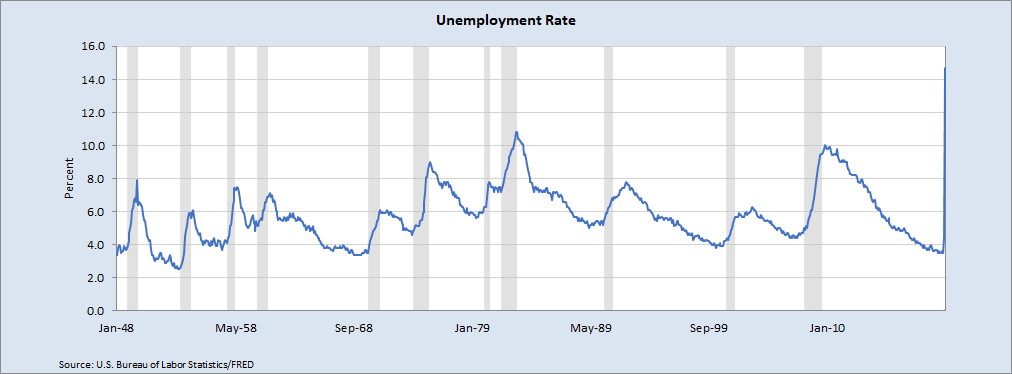
\includegraphics[width=1\linewidth]{Imagenes/Desempleo_USA_G}}
	\caption{\textbf{\textit{Tendencia del desempleo mensual de los EE.UU. hasta abril 20}} {\small La tendencia se muestra hacia hacia el incremento al mes de abril, con fuertes impactos en sectores claves de la economía. Fuente:  \href{https://www.govinfo.gov/app/collection/econi/2020/03/7}{https://www.govinfo.gov/app/collection/econi/2020/03/7}}
	} 
	\label{fig:4}
	
\end{figure}


\begin{figure}[H]
	\centering
	\resizebox{17 cm}{!} { 
	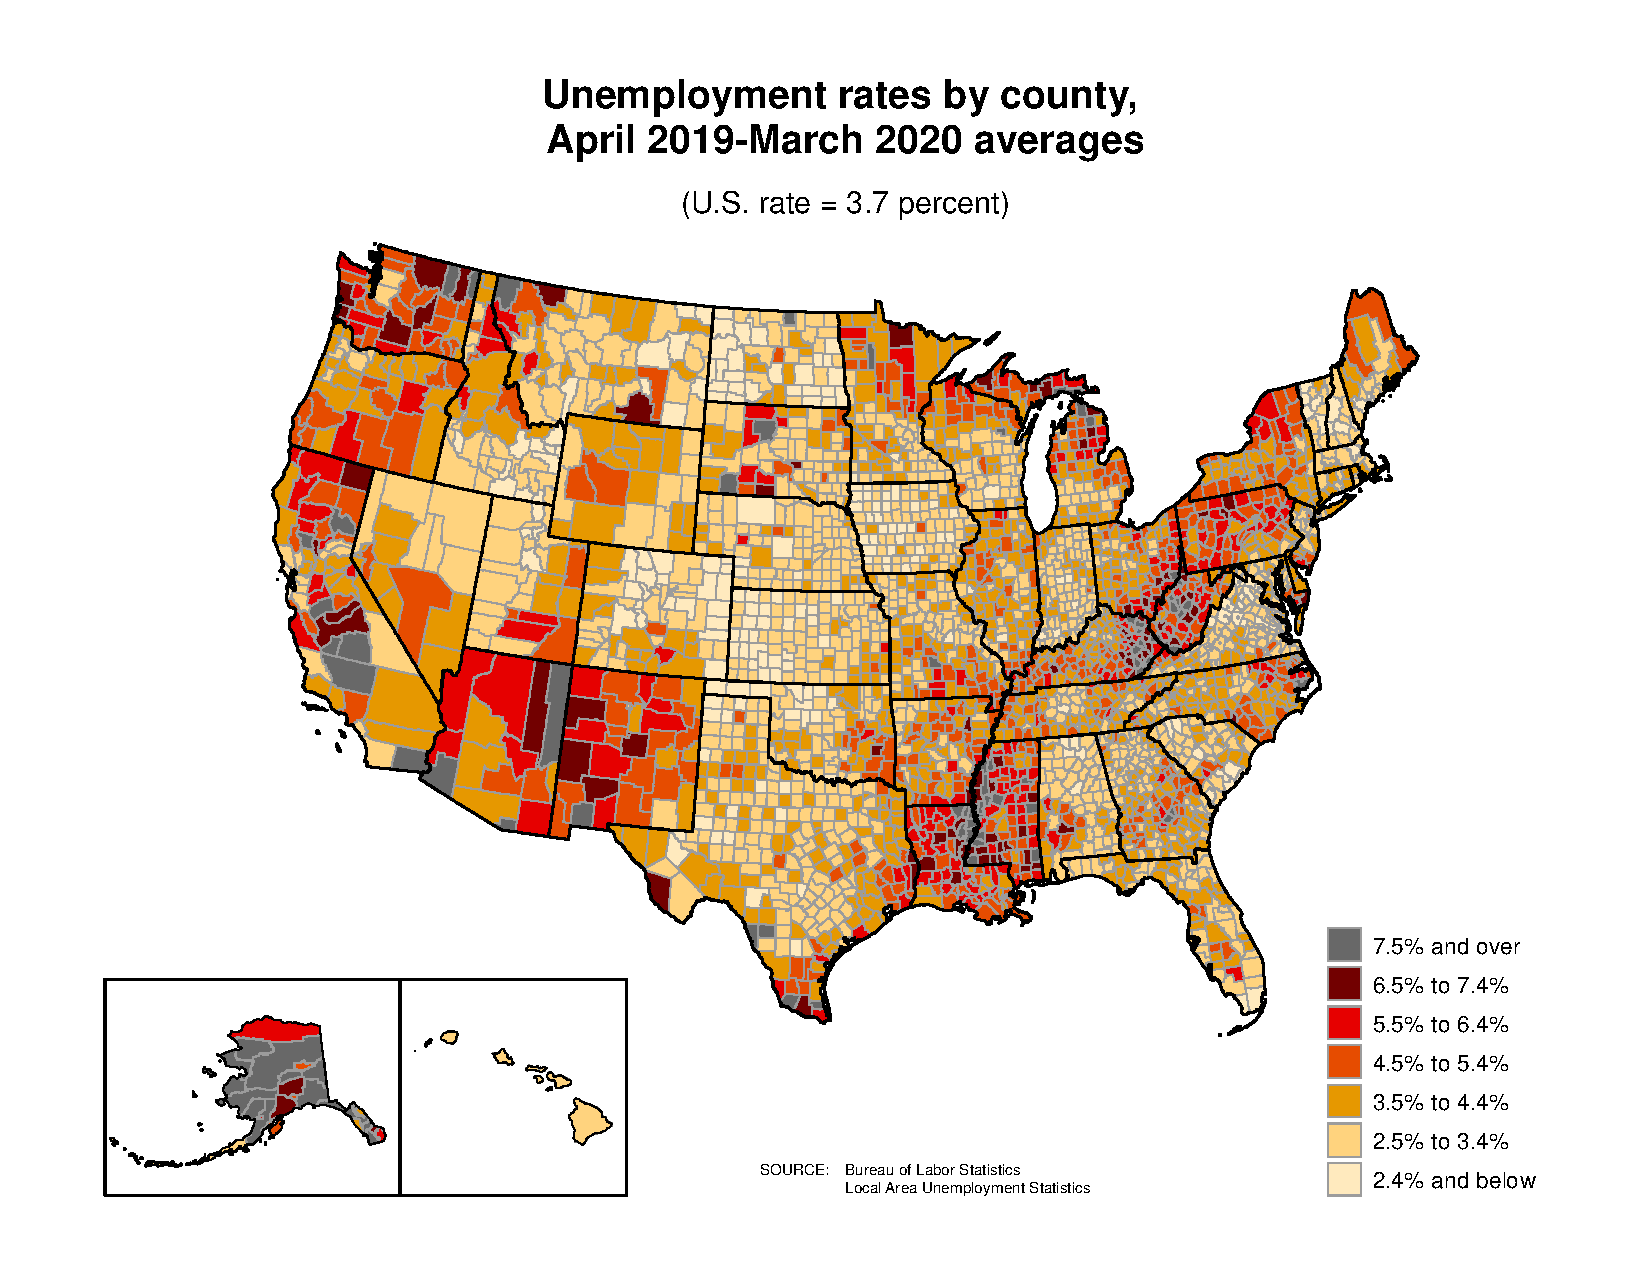
\includegraphics[width=1\linewidth]{Imagenes/Desempleo_USA}}
	\caption{\textbf{\textit{Mapa de los EE.UU. que muestra la concentración del desempleo a marzo 2020 por condados y ciudades.}}
	{\small Aproximadamente 3,192 condados o ciudades según tasas de desempleo por rangos. Fuente:  \href{https://www.govinfo.gov/app/collection/econi/2020/03/7}{https://www.govinfo.gov/app/collection/econi/2020/03/7}}
	} 
	\label{fig:5}
	
\end{figure}
  
Pero como se encuentra el impacto en el desempleo latino que es el que más preocupa por sus efectos en el envió de las remesas, este reportó una situación del $18.9 \textperthousand$ de desocupados, tal como se observa en la Figura No.\eqref{fig:6} aproximadamente $5.2$ millones de latinos o hispanos fueron desprendidos del mercado laboral ; desde marzo el desempleo paso de $807$ mil a $2.5$ millones de hombres de edades de entre 20 años o mayores, sin embargo el desempleo esta golpeando mayormente a las mujeres de ese mismo tramo de edades con una tasa del $20.2 \textperthousand$, el desempleo más joven en edades entre $16-19$ años sufrió una caída del $35.8 \textperthousand$.

\begin{figure}[H]
	\centering
	\resizebox{16.5 cm}{!} { 
		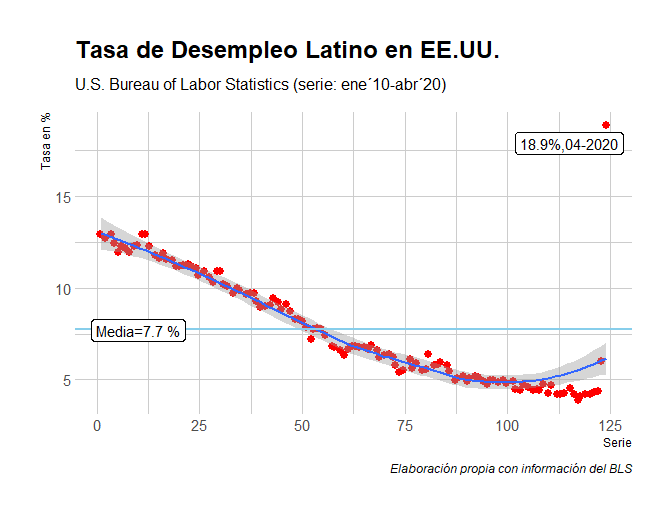
\includegraphics[width=1\linewidth]{Imagenes/TasaDeLa}}
	\caption{\textbf{\textit{Tendencia de la Tasa de Desempleo Hispano}}
		{\small Serie construida desde enero 2010 a abril 2020, la tasa de desempleo de las mujeres fue la más acentuada con el $20.2 \textperthousand$ Fuente: Elaboración propia con información de \href{https://www.bls.gov/news.release/empsit.t03.htm}{https://www.bls.gov/news.release/empsit.t03.htm}}
	} 
	\label{fig:6}
	
\end{figure}

La media mensual del desempleo se movió desde 2010 en $7.7\textperthousand$ y venía en descenso,  sin embargo la crisis del Covid-19 lo ha disparado fuertemente, desde enero $2020$ los hispanos empleados ascendían a $28.3$ millones de latinos y este dato bajo a $22.5$ millones, esto tendrá un impacto importante en las economía del mismo EE.UU. y los países de destino de las remesas a donde las dirigen los compatriotas residentes en USA. En términos absolutos en la siguiente tabla No.\eqref{Tabla 3} puede observar cuantos empleos se han perdido por mes, es muy probable que entre el mes de marzo y abril existan $7.03$ millones de latinos en estatus de desocupados.


\begin{table}[H]
	\centering
	\caption{\textbf{Cantidad de Desempleados Hispanos de EE. UU. en Miles (serie: ene10 - abr20) }}
	\label{Tabla 3}
	\resizebox{17cm}{!} { 
		\begin{tabular}{lcccccccccccc} \toprule			
			\textbf{Años}	&	\textbf{Ene}	&	\textbf{Feb}	&	\textbf{Mar}	&	\textbf{Abr}	&	\textbf{May}	&	\textbf{Jun}	&	\textbf{Jul}	&	\textbf{Ago}	&	\textbf{Sep}	&	\textbf{Oct}	&\textbf{	Nov}	&\textbf{	Dic}	\\  \midrule
			2010	&	2,930	&	2,879	&	2,931	&	2,830	&	2,722	&	2,783	&	2,772	&	2,731	&	2,827	&	2,801	&	2,941	&	2,952	\\ 
			2011	&	2,796	&	2,650	&	2,629	&	2,698	&	2,631	&	2,614	&	2,558	&	2,573	&	2,595	&	2,625	&	2,600	&	2,580	\\ 
			2012	&	2,566	&	2,639	&	2,551	&	2,499	&	2,665	&	2,680	&	2,490	&	2,456	&	2,385	&	2,449	&	2,421	&	2,357	\\ 
			2013	&	2,380	&	2,400	&	2,257	&	2,204	&	2,248	&	2,247	&	2,345	&	2,303	&	2,190	&	2,254	&	2,180	&	2,072	\\ 
			2014	&	2,072	&	2,059	&	1,981	&	1,816	&	1,939	&	1,971	&	1,963	&	1,896	&	1,732	&	1,760	&	1,703	&	1,641	\\ 
			2015	&	1,745	&	1,758	&	1,761	&	1,790	&	1,779	&	1,767	&	1,800	&	1,732	&	1,622	&	1,661	&	1,674	&	1,628	\\ 
			2016	&	1,533	&	1,446	&	1,472	&	1,634	&	1,495	&	1,583	&	1,460	&	1,522	&	1,739	&	1,552	&	1,551	&	1,592	\\ 
			2017	&	1,564	&	1,511	&	1,367	&	1,398	&	1,403	&	1,327	&	1,415	&	1,409	&	1,415	&	1,331	&	1,310	&	1,364	\\ 
			2018	&	1,380	&	1,375	&	1,401	&	1,363	&	1,380	&	1,291	&	1,264	&	1,318	&	1,299	&	1,249	&	1,297	&	1,268	\\ 
			2019	&	1,400	&	1,248	&	1,357	&	1,198	&	1,197	&	1,252	&	1,305	&	1,213	&	1,137	&	1,203	&	1,236	&	1,231	\\ 
			2020	&	1,275	&	1,322	&	1,771	&	5,263	&		&		&		&		&		&		&		&		\\  \bottomrule
			
			
		\end{tabular} 
		
	}
	{\small \text{Fuente:Elaboración propia conforme a datos de \href{https://www.bls.gov/webapps/legacy/cpsatab3.htm}{https://www.bls.gov/webapps/legacy/cpsatab3.htm} }}
	
\end{table}

Los sectores económicos más impactados por el desempleo tal como se menciono anteriormente, se encuentran: El Ocio y hospitalidad, con una tasa de desocupación del $39.3\textperthousand$ que emplea a más de $3,5$ millones de latinos, le sigue Otros servicios con una tasa de desempleo del $23.0\textperthousand$ y ocupa a $1.5$ millones de hispanos, Comercio mayorista y minorista emplea a $3.5$ millones de latinos y reporta una tasa de desempleo del $17.1\textperthousand$, el sector construcción es muy importante para el empleo latino, solo este sector emplea a $3.4$ millones de personas, pero su desempleo ha logrado un $16.6\textperthousand$, es importante resaltar que la industria que más hispanos contrata es Servicios de educación y salud con un empleo estimado de $4.8$ millones de latinos, pero es el décimo sector más golpeado con el desempleo con un $10.9\textperthousand$; lo sustancial es inferir que muchos sectores y sub-sectores de la economía de EE.UU. que emplean una importante cuantía de personal latino o hispano, han sido fuertemente golpeados con el desempleo generado por las medidas de cierre por la crisis del Covid-19, tal como se observa en la Tabla No. \eqref{Tabla 4}.


\begin{table}[H]
	\centering
	\caption{\textbf{Cantidad de personas por estatus de empleo según principales sectores y sub-sectores económicos, empleo latino estimado por tasa ocupación en EE. UU. en Miles (año 2019 - abr 2020) }}
	\label{Tabla 4}
	\resizebox{17cm}{!} { 
		\begin{tabular}{lcccc} \toprule			
				&	\textbf{Empleados}	&	\textbf{Tasa Empleados} 	&	\textbf{Empleados}	&	\textbf{Tasa Desempleados}	\\ 
			\textbf{Sectores}	&	\textbf{Totales 2019}	&	\textbf{Latinos 2019}	&	\textbf{Latinos 2019}	&	T\textbf{otal abril 2020}	\\  \midrule
			Ocio y hospitalidad	&	14,643	&	24.0	&	3,514	&	39.3	\\ 
			Otros servicios	&	7,617	&	19.9	&	1,516	&	23.0	\\ 
			Comercio mayorista y minorista	&	19,742	&	18.1	&	3,573	&	17.1	\\ 
			Construcción	&	11,373	&	30.4	&	3,457	&	16.6	\\ 
			Agricultura, silvicultura, pesca y caza.	&	2,425	&	27.5	&	667	&	15.6	\\ 
			Productos duraderos	&	9,970	&	14.8	&	1,476	&	15.1	\\ 
			Transporte y utilidades	&	8,991	&	18.8	&	1,690	&	13.5	\\ 
			Fabricación	&	15,741	&	16.8	&	2,644	&	13.2	\\ 
			Información	&	2,766	&	12.5	&	346	&	11.0	\\ 
			Servicios de educación y salud.	&	35,894	&	13.5	&	4,846	&	10.9	\\ 
			Minería, canteras y extracción de petróleo y gas.	&	750	&	20.1	&	151	&	10.2	\\ 
			Bienes no duraderos	&	5,771	&	20.2	&	1,166	&	10.2	\\ 
			Servicios profesionales y empresariales.	&	19,606	&	16.0	&	3,137	&	9.8	\\ 
			Trabajadores del gobierno	&	7,225	&	12.5	&	903	&	9.4	\\ 
			Actividades financieras	&	10,765	&	12.9	&	1,389	&	5.4	\\  \bottomrule
			
			
			
						
		\end{tabular} 
		
	}
	{\small \text{Fuente:Elaboración propia conforme a datos de \href{https://www.bls.gov/webapps/legacy/cpsatab3.htm}{https://www.bls.gov/webapps/legacy/cpsatab3.htm} }}
	
\end{table}

%-----------------------------------------
\section{METODOLOGÍA}

%---------------
\subsection{Planteamiento General de la Metodología de la Investigación}

La metodología que se aplica en la presente investigación se desarrolla en dos partes: la primera consiste en estimar un modelo sencillo de regresión simple por el método de mínimos cuadrados para realizar la proyección de la cuantía de remesas para el segundo trimestre (abril-junio 2020) explicada por el comportamiento o tendencia del PIB trimestral de USA, ajustado por las tasas de contracción económica ya determinadas y pronosticadas por modelos económétricos realizados por expertos del mismo EE.UU. y a través de esta estimación, tener una referencia del nivel en que se verán reducidas las transferencias familiares hacia el país; las fuentes de información empleadas fueron: Govinfo.gov \footnote{\href{https://www.govinfo.gov/app/collection/econi/2020/03/7}{https://www.govinfo.gov/app/collection/econi/2020/03/7}} e informe de remesas del Banco Central de Reserva de El Salvador BCR
\footnote{\href{https://www.bcr.gob.sv/esp/index.php?option=com_wrapper&view=wrapper&Itemid=469}{https://bit.ly/2LpgvUB}} .\\

En segundo termino, ya conocida la reducción específica de la cuantía de remesas, se ajustará con ello el monto de la ayuda acumulada en los ingresos familiares reportados en la Encuesta de Hogares de Propósitos Múltiples ya que se anualizan y posteriormente se prorratean de manera mensual y de forma percapita para calcular la pobreza, comparando dicho monto con el costo de la canasta básica alimentaria CBA, en la investigación se reajustará esos nivel de ingreso por pérdida de transferencia monetaria y se definirán nuevos cálculos de pobreza a 2018, para obtener un proxi o escenario de recomposición de la pobreza para conocer a donde estaría golpeando mayoritariamente, ante el efecto de una contracción económica de USA y su impacto en los empleos latinos; adicional a ello se hará un escenario de calculo de la pobreza por medio de los índices FGT (Foster,Greer y Thorbecke) creados por James Foster, Joel Greer y Erik Thorbecke, encontrando mayor referencia teórica en \cite{Foster} y \cite{feres2001enfoques} todo lo anterior con el objetivo de extrapolar la incidencia, brecha y severidad de la pobreza para los 50 municipios auto-representados de la EHPM 2018.\\

\textbf{Principales pasos metodológicos llevados a cabo:}
\begin{itemize}
	\item Preparación de la base de datos y la serie del PIB trimestral de EE:UU. y las cuantías de las remesas.
	\item Se diseño y ejecuto el modelo de regresión lineal simple con mínimos cuadrados para estimar la cuantía de remesas explicada por el crecimiento o caída del PIB de EE.UU..
	\item Se desarrollo las prueba de los supuestos del modelo para pronosticar la cuantía de remesas trimestrales.
	\item Se prepararon las bases de los 50 municipios auto-representados para calcular los indicadores FGT de pobreza.
	\item Calculo de los indicadores FGT de pobreza para los 50 municipios y desarrollo de las estimaciones y sus variaciones.
	
\end{itemize}

A continuación en la siguiente sección se explica con mayor detalle y rigurosidad técnica la propuesta del modelo de regresión lineal simple para definir los montos de remesas vía explicación de la tendencia del PIB de EE.UU. y la cuantificación de los indices FGT para medir la pobreza.


\newpage

%---------------------
\subsection{Teoría del Modelo de Regresión Simple}


Para la construcción del modelo se empleo una potente herramienta de análisis estadístico como lo es el lenguaje R. Se corrió el programa para estimar los parámetros de la ecuación, las pruebas paramétricas para corroborar los supuestos  y se construyeron las gráficas de los errores o residuales para corroborar las pruebas, para una mejor referencia del lenguaje R, favor consultar \cite{wickham2016r} .\\

Los pasos en el proceso de la determinación del modelo fueron los siguientes:

\begin{enumerate}
	\item Preparación de la base de datos con los principales indicadores PIB EE.UU. y Remesas de forma trimestral.
	\item Revisión de la consistencia de la base de datos en la serie de datos establecida.
	\item Análisis de las correlaciones parciales bivariadas para identificar cuales de ellas pueden determinar las variables explicadas y explicativas.
	\item Por ser el modelo simple se seleccionan las variable explicativa fue el PIB EE.UU. se desarrollaron pruebas con otras variables pero la prueba de los supuestos dieron presencia de colinealidad a pesar de desarrollar las transformaciones respectivas.
	\item Corrida del modelo con las variables con mayores correlaciones entre sí.
	\item Se corren todas las pruebas de los supuestos del modelo para saber su robustez para estimar.
	\item Se analizan los escenarios de estimación de la variable explicada con ajustes arbitrarios a coeficientes estimados por otros modelos econométricos para la estimación del crecimiento del PIB de USA.	
	
\end{enumerate}

Como en todo modelo, se deben determinar los supuestos teóricos para una correcta interpretación de los estimados:	


\begin{itemize}
	\item \textbf{El modelo no es completamente concluyente:} es importante destacar este hecho debido a que se debe continuar ejecutando más pruebas de ajuste y revisión de variables que provienen de indicadores económicos que por lo general a lo largo del tiempo pueden sufrir cambios por la misma dinámica económica. 
	\item \textbf{El resto de todas las variables permanecen constantes:} las estimaciones resultantes por el modelo cuentan con el supuesto de que el resto permanecen constantes y solo se encuentran influenciadas por el error aleatorio.
	\item \textbf{Otras variables fueron excluidas del modelo por la alta correlación con las remesas} se excluyeron variables debido a la alta correlación entre ellas lo que generó problemas de multicolinealidad, prueba que viola uno de los supuesto técnicos, a pesar de las transformaciones fue necesario extraerlas del modelo, mejorando su bondad de ajuste.
	\item \textbf{El presente modelo sirve como una referencia general para estimar en que porcentaje suben o caen los montos en remesas:} la disponibilidad de información de los indicadores macroeconómicos de EE.UU. es muy buena y esto puede afinarse aún más con la inclusión de más variables, sin embargo para la finalidad de la investigación se desarrollo solo para observar el cambio de tendencia o pendiente de las remesas explicada por la economía de USA. 
	
\end{itemize}


Este apartado toma las referencias de las citas y marco teórico de \cite{mendenhall1994estadistica} y \cite{anderson2012estadistica} para exponer los aspectos técnicos del modelo de método de minimos cuadrados para una regresión lineal simple pero con posibilidad de ampliarse a una múltiple. Un procedimiento para estimar los parámetros de cualquier modelo lineal, el método de mínimos cuadrados, se puede ilustrar con sólo ajustar una recta a un conjunto de puntos. Suponga que deseamos ajustar el modelo:

\begin{center}
	{\large $\displaystyle E(Y)=\beta_{0}+\beta_{1} \; x$}
\end{center}

al conjunto de puntos que se muestra para el modelo. [La variable independiente $x$ podría
ser $w2$ o $(w)1/2$ o $ln$ $w$, etc., para alguna otra variable independiente $w$.] Esto es, postulando
que $Y = \beta_{0} + \beta1_{1}\; x  + \epsilon$, donde $\epsilon$ tiene alguna distribución de probabilidad con $E(\epsilon) = 0$. Si $\hat{\beta}_{0}$ y Si $\hat{\beta_{1}}$ son estimadores de los parámetros $\beta_{0} y \beta_{1}$, entonces $\hat{Y} = \hat{\beta_{0}}+\hat{\beta_{1}}x$ es claramente un
estimador de $E(Y)$.\\

El procedimiento de mínimos cuadrados para ajustar una recta que pase por un conjunto de $n$ puntos es semejante al método que podríamos usar si ajustamos una recta a simple vista; esto es, deseamos que las diferencias entre los valores observados y los puntos correspondientes en la recta ajustada sean “pequeñas” en un sentido general. Una forma cómoda de lograr esto y que proporciona estimadores con buenas propiedades, es minimizar la suma de cuadrados de las desviaciones verticales a partir de la recta ajustada (vea las desviaciones indicadas en la figura \eqref{fig:7}.


\begin{figure}[H]
	\centering
	\caption{\textbf{Ajuste de una recta que pasa por un conjunto de puntos}}
	\label{fig:7}
	\resizebox{9cm}{!} { 
		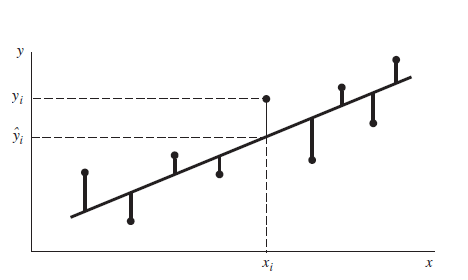
\includegraphics[width=1\linewidth]{Imagenes/Img_02}
	}
	{\scriptsize \text{Fuente: Estadística Matemática con Aplicaciones.Wackerly y Sheafer }}
\end{figure}

Entonces, si	

\begin{center}
	{\large $\hat{y}_{i} =\hat{\beta_{0}}+\hat{\beta_{1}}x_{1}$}
\end{center}

es el valor pronosticado del i-ésimo valor $y$ (cuando $x = x_{i}$), entonces la desviación (a veces llamada error) del valor observado de $y_{i}$ a partir de $\hat{y}_{i} =\hat{\beta_{0}}+\hat{\beta_{1}}x_{1}$ es la diferencia $y_{i} - \hat{y}_{i}$ y la suma de los cuadrados de las desviaciones a minimizar es

\begin{center}
	{\large $\displaystyle SEE=\sum_{i=1}^{n} \; \left(y_{i}-\hat{y_{1}} \right)^{2}= \sum_{i=1}^{n} \; \left[y_{i} -\left( \hat{\beta_{0}} + \hat{\beta_{1}}x_{i} \right)  \right]^{2}$}
\end{center}

La cantidad \textbf{SSE} también recibe el nombre de suma de cuadrados del error por razones que más adelante se harán evidentes. Si la \textbf{SSE} tiene un mínimo, ocurrirá para valores de $\beta_{0}$ y $\beta_{1}$ que satisfagan las ecuaciones,$\partial SSE/\partial  \hat{\beta_{0}} =\;0$ y $\partial SSE/\partial  \hat{\beta_{1}} =\;0$. Tomando las derivadas parciales de la \textbf{SSE} con respecto a
$\hat{\beta_{0}}$ y $\hat{\beta_{1}}$ e igualando a cero, obtenemos:\\



\begin{center}
$
\dfrac{\partial SSE}{\partial \hat{\beta_{0}} }=\dfrac{\partial \left\lbrace \sum_{i=1}^{n} \; \left[ y_{i}-\left( \hat{\beta_{0}} + \hat{\beta_{1}}x_{i} \right)  \right]^{2} \right\rbrace }{\partial\hat{\beta_{0}}}=-\sum_{i=1}^{n} 2 \left[y_{i} -\left( \hat{\beta_{0}} + \hat{\beta_{1}}x_{i} \right)  \right]
$
$=\;-2\left(\sum_{i=1}^{n}y_{i}-n\hat{\beta_{0}}-\hat{\beta_{1}}  \sum_{i=1}^{n} x_{i}\right)=\;0$	
\end{center}

y


\begin{center}
$
\dfrac{\partial SSE}{\partial \hat{\beta_{1}} }=\dfrac{\partial \left\lbrace \sum_{i=1}^{n} \; \left[ y_{i}-\left( \hat{\beta_{0}} + \hat{\beta_{1}}x_{i} \right)  \right]^{2} \right\rbrace }{\partial\hat{\beta_{1}}}=-\sum_{i=1}^{n} 2 \left[y_{i} -\left( \hat{\beta_{0}} + \hat{\beta_{1}}x_{i} \right)  \right]x_{1}
=\;-2\left(\sum_{i=1}^{n}x_{i} y_{i}-\hat{\beta_{0}}  \sum_{i=1}^{n}x_{i}-\hat{\beta_{1}}\sum_{i=1}^{n} x^{2}_{i}\right)=\;0$	
\end{center}



Las ecuaciones $\partial SSE/\hat{\beta_{0}} = 0$ y $\partial SSE/\hat{\beta_{1}} = 0$ se denominan ecuaciones de mínimos cuadrados para estimar los parámetros de una recta. Las ecuaciones de mínimos cuadrados son lineales en $\hat{\beta_{0}}$ y $\hat{\beta_{1}}$ y por tanto pueden resolverse simultáneamente.Puede verificar que las soluciones son:




\begin{center}

$
{\large \hat{\beta_{1}}=\dfrac{\sum_{i=1}^{n}\left(x_{i}-\bar{x} \right) \left(y_{i}-\bar{y} \right)}{\left(x_{i}-\bar{x} \right)^{2}} = \dfrac{\sum_{i=1}^{n}x_{i}y_{i}-\dfrac{1}{n}\sum_{i=1}^{n}x_{i} \sum_{i=1}^{n}y_{i}}{\sum_{i=1}^{n}x^{2}_{i}-\dfrac{1}{n}\left( \sum_{i=1}^{n}x_{i}\right)^{2}}}
$


$
{\large \hat{\beta_{0}}=\bar{y}-\hat{\beta_{1}}\bar{x}}
$
\end{center}



Además, se puede demostrar que la solución simultánea para las dos ecuaciones de mínimos cuadrados da valores de $\hat{\beta_{0}}$ y $\hat{\beta_{1}}$ que minimizan la SSE. Dejamos esto para que lo compruebe. Las expresiones son las siguientes:



\begin{center}

$
{\large \sum_{i=1}^{n}\left(x_{i}-\bar{x} \right) \left(y_{i}-\bar{y} \right) \; y \; \sum_{i=1}^{n} \left(x_{i}-\bar{x} \right)^{2}}
$
\end{center}



Estas expresiones se usan para calcular $\hat{\beta_{1}} $ se encuentran a menudo en el desarrollo de modelos de regresión lineal simple. La primera de éstas se calcula al sumar productos de valores $x$ menos su media y valores $y$ menos su media, denotando esta cantidad
por $S_{xy}$. Del mismo modo, denotaremos la segunda cantidad por $S_{xx}$ porque se calcula al sumar productos que contienen únicamente los valores $x$. Los estimadores de mínimos cuadrados para el modelo de regresión lineal simple:


\begin{center}

$
{\large 1. \; \hat{\beta_{1}}=\dfrac{S_{xy}}{S_{xx}}, \; donde \; S_{xy}=\sum_{i=1}^{n}\left(x_{i}-\bar{x} \right) \left(y_{i}-\bar{y} \right) \; y\; S_{xx}\;= \sum_{i=1}^{n} \left(x_{i}-\bar{x} \right)^{2}}  
$

$
{\large 2.\; \hat{\beta_{0}}=\bar{y}-\hat{\beta_{1}}\bar{x} }
$
\end{center}


\newpage

%-------------------
\subsection{Índice FGT}

El índice FGT propuesto por James Foster, Joel Greer y Erik Thorbecke, \cite{navarro2007indice}
es un índice de carencias en el consumo privado que toma como referencia una
determinada línea de pobreza individual, de manera general obtenida ésta a
partir de un salario mínimo diario o el costo de una CBA, de la población total y de la población
económicamente activa. Con esta información es posible calcular la proporción
de la población en condiciones de pobreza extrema, definida como el número de
habitantes cuyo ingreso se encuentra por debajo de la línea de pobreza sobre la
población total. Mientras el índice FGT adquiera valores superiores, ésto será
reflejo de un deterioro en el nivel de satisfacción del consumo individual. Para el calculo de los índices FGT en la investigación se utilizó un corte o un $z=$ US$\$$ 106.8, lo que representa el doble costo de una canasta básica alimentaria CBA en la zona urbana como estandard.\\


Si bien típicamente las medidas más utilizadas han sido el “índice de recuento” y la “brecha de ingreso”, numerosas alternativas han sido propuestas a partir de la crítica de \cite{sen1985well}. A su vez, \cite{Foster} señala que las medidas existentes muestran distintas dimensiones de la pobreza, por lo que ninguna de ellas es mejor o peor en todos los casos, así, el índice de recuento mide el “predominio” de la pobreza, la brecha de ingreso da cuenta de la “profundidad” de la pobreza, y las medidas sugeridas posteriormente indican la “severidad” de la pobreza. Éste grupo de medidas pertenecen a la familia de índices paramétricos propuesto por Foster, Greer y Thornbeck, estos índices pueden interpretarse como una brecha de pobreza en la que se le asigna mayor peso relativo a los individuos mientras más lejos se encuentren de la línea de pobreza. Como se puede observar en la siguiente tabla No. \eqref{Tabla 5}

\begin{table}[H]
	\centering
	\caption{\textbf{Indicadores Foster, Greer y Thorbecke FGT }}
	\label{Tabla 5} 
	\resizebox{16cm}{!} {
		\begin{tabular}{lcc} \toprule \\ 									
			\textbf{Indicador}	&	\textbf{Formula}	&	\textbf{Concepto}\\ \midrule
			\textbf{Índice de Recuento}& $H =\frac{q}{n}$&  $\infty= 0$, esta medida es igual al índice de recuento \\&& $P_{\infty-0} $;Este índice mide la proporción de personas\\&& que se encuentran bajo la línea de pobreza\\\\
			\textbf{Índice de Brecha}& $P_{\infty}=\frac1{n}\sum_{i=1}^q \left(\frac{z-y_{i}}z\right)^\infty$ &  $\infty= 1$,se obtiene la brecha de pobreza \\&& $P_{\infty-1} $;Indica la distancia promedio de las personas\\&& pobres a la línea de pobreza, ponderado por la incidencia\\&& de pobreza\\\\
			\textbf{Índice de Severidad} & $P_{\infty}=\frac1{n}\sum_{i=1}^q \left(\frac{z-y_{i}}z\right)^\infty$ &  $\infty= 2$, se obtiene la severidad de la pobreza\\&& $P_{\infty-2} $; Otorga más peso a las personas muy pobres\\&& En otras palabras, la severidad de la pobreza \\&&obtiene en cuenta la desigualdad entre los pobres
			
			\\ \bottomrule
			
		\end{tabular} 
	}
	{\scriptsize \text{Fuente:Foster and Thornbecke,A class of decomposable poverty measures,Econometrica: journal of the econometric society;1984}}
	
\end{table}

Con el calculo de éstos indicadores por municipio se podrá conocer la incidencia, brecha y severidad de la pobreza, proporcionando mayor luz hacia a donde se debe priorizar la ayuda Gubernamental hacia adentro de los 50 municipios auto-representados que la EHPM defnie por importancia y peso muestral asociado a concentraciones poblacionales, con la finalidad de establecer políticas de rescate o programas estatales para subsanar en parte los deficits en las transferencias monetarias desde el exterior.

%-----------------------------------------
\section{RESULTADOS DEL MODELO E INDICADORES FGT}
%-------------
\subsection{Resultados del Modelo de Regresión Lineal para Estimar Remesas}

A continuación se desarrolla el procedimiento del modelo de regresión simple para estimar el monto de las remesas a través de la variable explicada del PIB EE.UU., se ejecutan los pasos y las pruebas del modelo, a continuación su relación de tendencia gráfica y principales resultados, se puede observar su relación en la gráfica No. \eqref{fig:8} :

\begin{figure}[H]
	\centering
	\resizebox{16.5 cm}{!} { 
		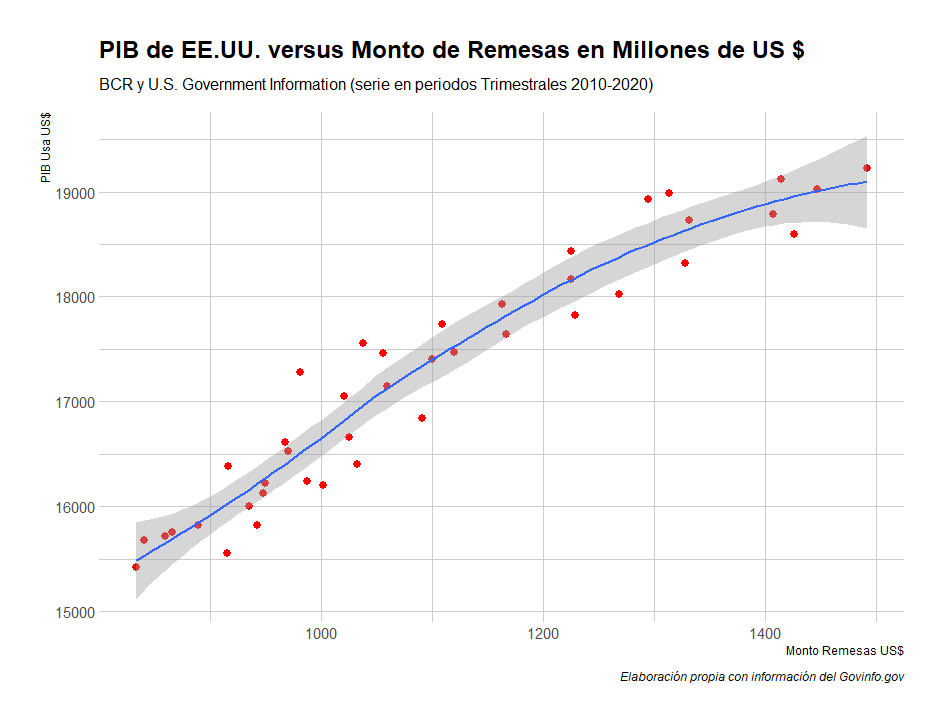
\includegraphics[width=1\linewidth]{Imagenes/Grafo_08}}
	\caption{\textbf{\textit{Tendencia del PIB de EE.UU. y Remesas.}}
		{\small Serie construida desde el trimestre I 2010 al Trimestre I 2020, El PIB muestra una tendencia al alza, similar al monto de las remesas, sin embargo estos se redujeron en US\$ $18,987.88$ y US\$$1,313.45$ respectivamente  Fuente: Elaboración propia con información de \href{https://www.govinfo.gov/}{https://www.govinfo.gov/}}
	} 
	\label{fig:8}
	
\end{figure}

Se denota en la gráfica de puntos la correlación entre la variable del PIB de USA y las remesas, esto explica su factibilidad de modelar en forma de regresión lineal simple, estimando que su correlación será alta, indicando que una de la variable puede explicar a la otra o viceversa, objetivo que se persigue, para medir el cambio de pendiente o cambio de signo que puede ser positivo o negativo, estimando la disminución en el monto de las remesas para el trimestre indicado. A continuación se observan las relaciones gráficas de cada una de las variables sometidas al modelo y sus respectivas correlaciones, observar su conformación en las siguientes Figuras\eqref{fig:9} y \eqref{fig:10}:

\begin{figure}[H]
	\centering
	\resizebox{12 cm}{!} { 
		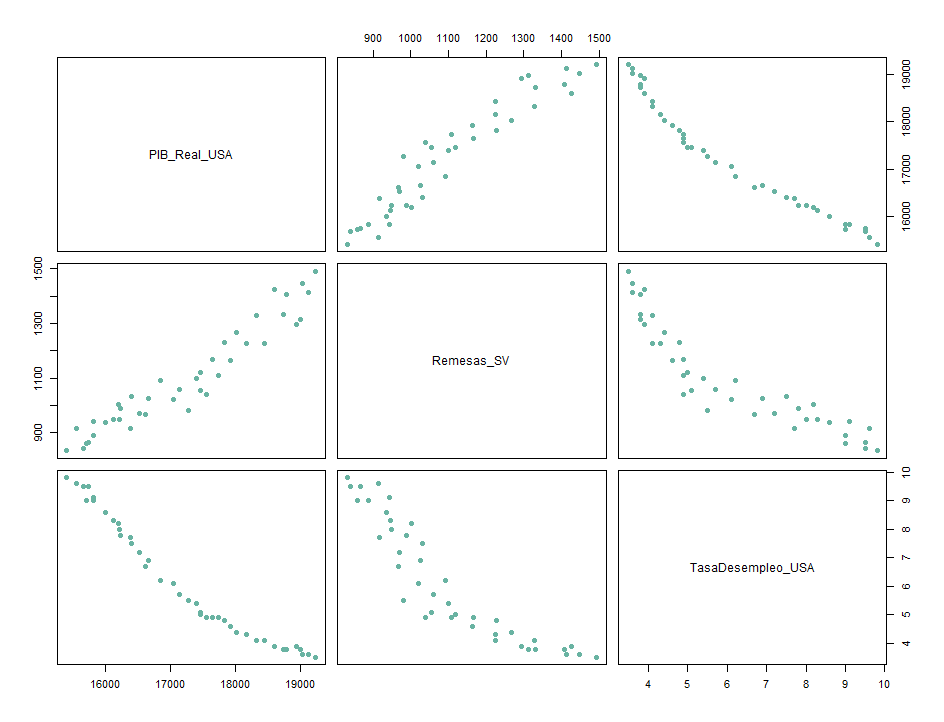
\includegraphics[width=1\linewidth]{Imagenes/Grafo_09}}
	\caption{\textbf{\textit{Relación gráfica del PIB de EE.UU., Remesas y Tasa de desempleo USA.}}
		{\small Serie construida desde el trimestre I 2010 al Trimestre I 2020, El PIB muestra una tendencia al alza o una relación positiva contra el monto de las remesas y contra la tasa de desemplo muestra una relación negativa, Fuente: Elaboración propia con información de \href{https://www.govinfo.gov/}{https://www.govinfo.gov/}}
	} 
	\label{fig:9}
	
\end{figure}


\begin{figure}[H]
	\centering
	\resizebox{12 cm}{!} { 
		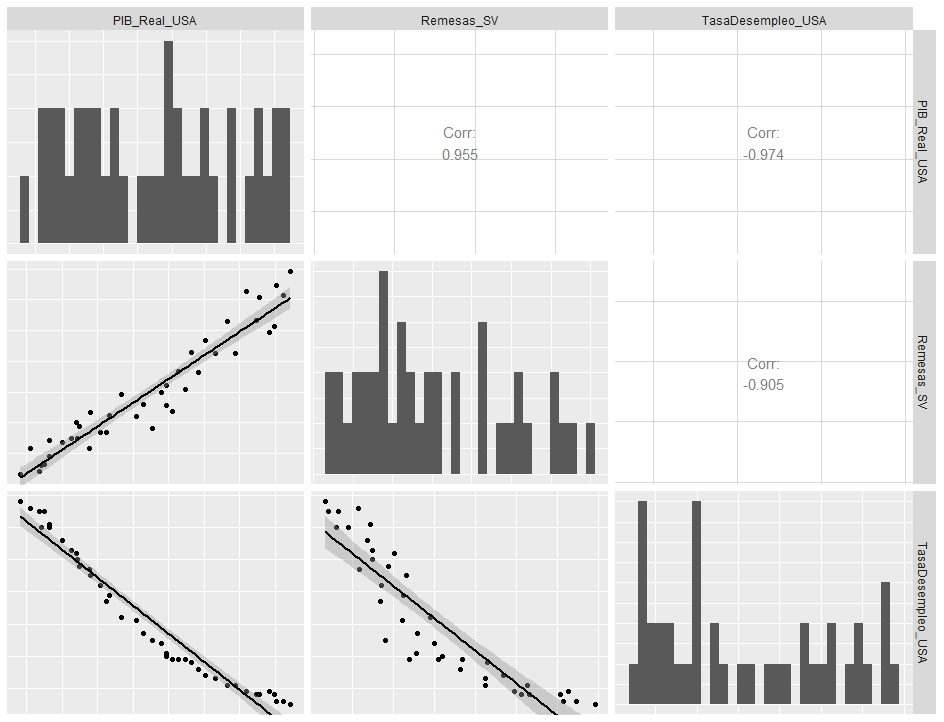
\includegraphics[width=1\linewidth]{Imagenes/Grafo_10}}
	\caption{\textbf{\textit{Tendencia del PIB de EE.UU. y Correlación contra Remesas y Tasa de desempleo USA.}}
		{\small Serie construida desde el trimestre I 2010 al Trimestre I 2020, El PIB muestra una correlación bastante fuerte a las remesas con $0.95$ y contra la Tasa de desempleo la correlación alcanza los $0.974$ Fuente: Elaboración propia con información de \href{https://www.govinfo.gov/}{https://www.govinfo.gov/}}
	} 
	\label{fig:10}
	
\end{figure}

A continuación se muestran resultados del resumen del modelo, estimación de los supuestos coeficientes y significancia, la Figura No. \eqref{fig:11} muestra los principales resultados: 

\begin{figure}[H]
	\centering
	\resizebox{10 cm}{!} { 
		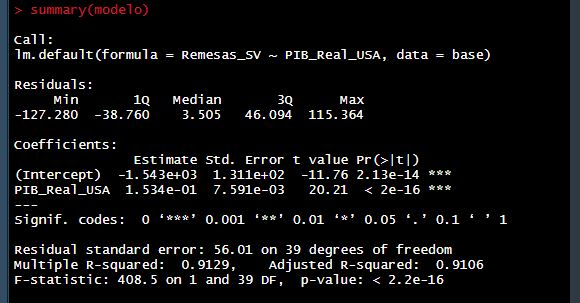
\includegraphics[width=1\linewidth]{Imagenes/Modelo}}
	\caption{\textbf{\textit{Resultados y resumen de las pruebas de significancia del modelo.}}
		{\small El modelo muestra significancia, con un $R^{2}$ ajustado de $91.06\textperthousand$.  y la prueba F es significativa lo que indica que $\beta \neq 0$.}
	} 
	\label{fig:11}
	
\end{figure}

Las pruebas de los supuestos del modelo se puede observar en la Figura No \eqref{fig:12}. 

\begin{figure}[H]
	\centering
	\resizebox{17 cm}{!} { 
		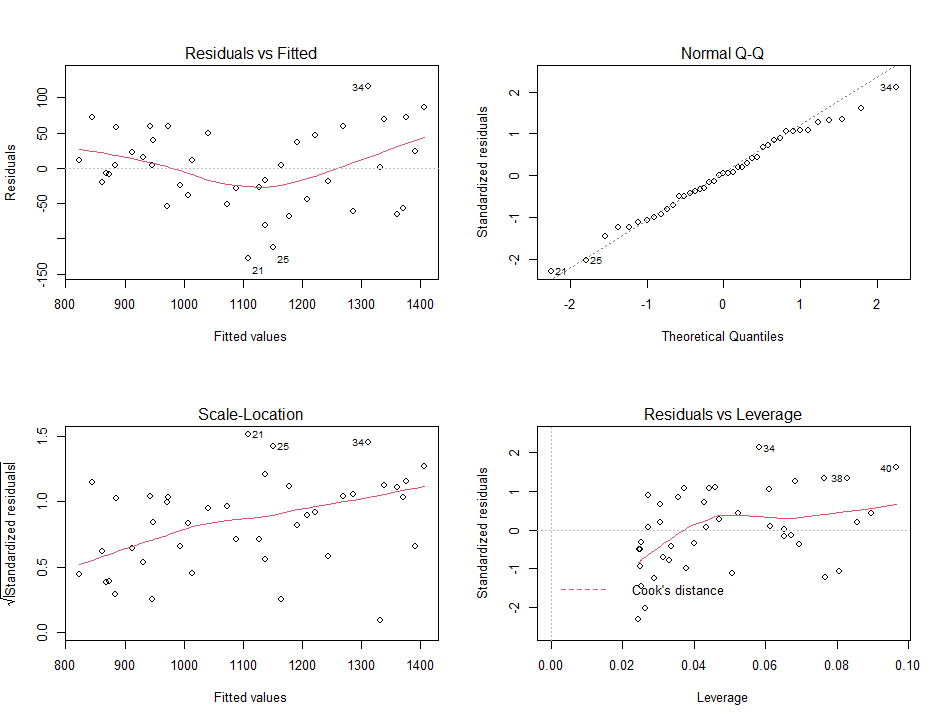
\includegraphics[width=1\linewidth]{Imagenes/PruebasModelo}}
	\caption{\textbf{\textit{Pruebas de los residuales comprobando los supuestos del modelo de forma gráfica.}}
		{\small Se desarrollaron las gráficas donde se muestra la tendencia y normalidad de los residuales.}
	} 
	\label{fig:12}
	
\end{figure}

Los coeficientes resultantes del modelo y las diferentes pruebas de normalidad de los residuales, se pueden observar en las siguientes Figuras \eqref{fig:13} y \eqref{fig:14}  :


\begin{figure}[H]
	\centering
	\resizebox{7 cm}{!} { 
		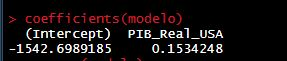
\includegraphics[width=1\linewidth]{Imagenes/Coeficientes}}
	\caption{\textbf{\textit{Resultados de los coeficientes del modelo.}}
		{\small Se muestra la constante en signo negativo y el valor que pondera el coeficiente.}
	} 
	\label{fig:13}
	
\end{figure}


\begin{figure}[H]
	\centering
	\resizebox{10 cm}{!} { 
		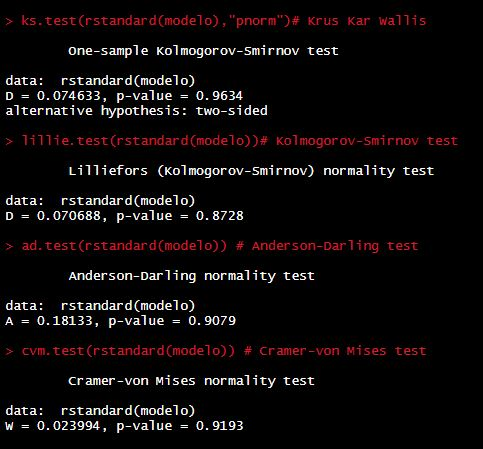
\includegraphics[width=1\linewidth]{Imagenes/Pruebas}}
	\caption{\textbf{\textit{Resultado de las diferentes pruebas de normalidad de los residuales del modelo.}}
		{\small Todos los resultados muestran que la tendencia de los residuales corroboran normalidad.}
	} 
	\label{fig:14}
	
\end{figure}


Posteriormente a desarrollar todas las pruebas de los supuestos del modelo se valida para realizar las estimaciones, la ecuación del modelo queda de la siguiente manera:\\


$
{\large \theta=-1542.69+\beta_{PibRealUsa}(0.1534)+\epsilon}
$
\\
\\
\textbf{a donde:}\\
$\theta$ = Monto Trimestral de Remesas en dólares\\
$\beta_{PibRealUsa}$ = PIB Real de los EE.UU. en dólares\\
$\epsilon $= Error aleatorio\\

{\large }


\newpage

Según la proyección del modelo econométrico de \cite{kozlowski2020scarring}  Julian Kozlowski, Laura Veldkamp y Venky Venkateswaran \footnote{\href{https://s3.amazonaws.com/real.stlouisfed.org/wp/2020/2020-009.pdf}{https://s3.amazonaws.com/real.stlouisfed.org/wp/2020/2020-009.pdf}}, el impacto en el escenario I es una contracción del $18\textperthousand$ para el PIB real de EE.UU. en el segundo trimestre 2020, lo que indica que si lo aplicamos al modelo estimado las remesas para el T2 tendría un resultado en su monto de US$\$$ 846.13 millones, es decir que estas se verán reducidas o mermadas en US$\$$ 467.32 millones con respecto al T1. El impacto de la contracción económica de EE.UU. por efectos del Covid-19, en un escenario fuerte de perdida de capital, representaría una caída del $18\textperthousand$ lo que a su vez afectaría el monto de las remesas, dando como resultado una reducción  por $35.6 \textperthousand$, se puede observar en la Figura No. \eqref{fig:15} la proyección de las remesas.

\begin{figure}[H]
	\centering
	\resizebox{16.5 cm}{!} { 
		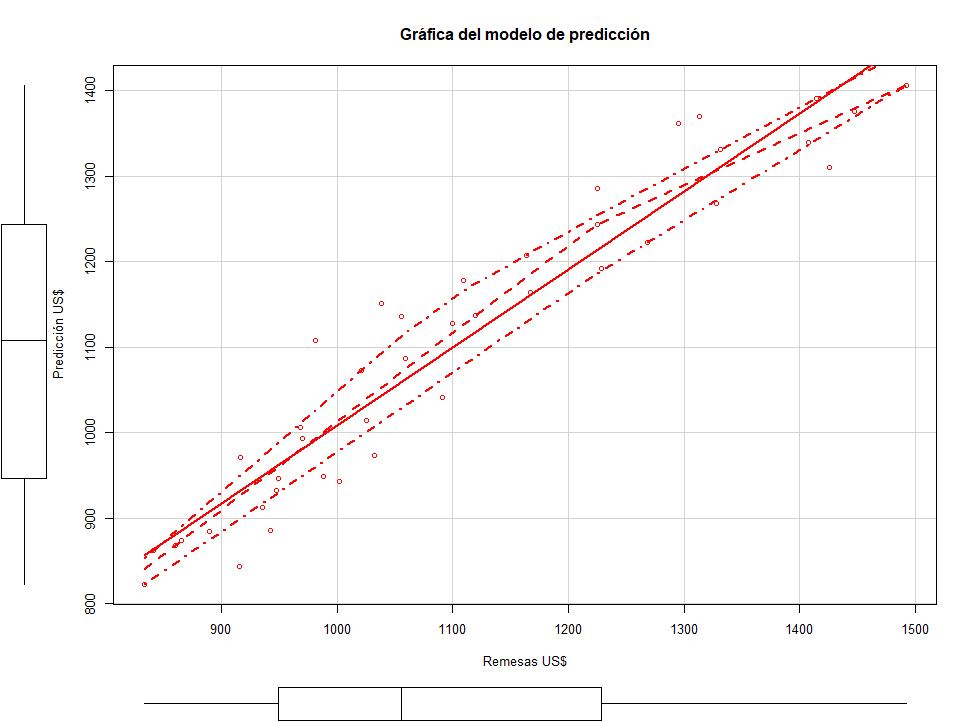
\includegraphics[width=1\linewidth]{Imagenes/Prediccion}}
	\caption{\textbf{\textit{Gráfica del modelo de predicción versus Remesas con sus respectivos intervalos.}}
		{\small Se muestra que la proyección presenta una relación o tendencia lineal.}
	} 
	\label{fig:15}
	
\end{figure}

Es importante hacer notar que el PIB EE.UU. ya había mostrado para el T1 una reducción del $-1.2 \textperthousand$,sumado al escenario de proyección de la contracción económica por $18.0 \textperthousand$, los impactos serán fuertes para las remesas en el T2, que también ya habían demarcado una caída en el T1 del $12.0 \textperthousand$, el modelo indica una reducción significativa de las remesas, por un $35.6 \textperthousand$.

\newpage
%-------------------------
\subsection{Recomposición de la Pobreza en General}

El modelo construído indica una pérdida de US$\$$ 467.32 millones en remesas, como resultado de una contracción del  $18\textperthousand$ para el PIB real de EE.UU. en el segundo trimestre 2020, derivando en una alta tasa de desempleo que al mes de abril se situaba en $14.7 \textperthousand$ y en $18.9 \textperthousand$, para la comunidad latina, tal como ya fue analizado, los sectores económicos más importantes de EE.UU. y que presentan la mayor contratación de población hispana, fueron afectados ampliamente; dicho impacto dado por la contracción y ahora ya consolidada recesión económica de USA, a niveles  superiores e históricos a las pérdidas de la gran depresión de 1932, se convierte en una recomposición en la pobreza nacional, tal como se observa en la siguiente tabla No. \eqref{Tabla 6}: 

\begin{table}[H]
	\centering
	\caption{\textbf{Recomposición de la condición de pobreza por Hogares y Personas }}
	\label{Tabla 6}
	\resizebox{10.5cm}{!} { 
		\begin{tabular}{lccc} \toprule			
		\textbf{Ítems}	&	\textbf{Hogares}	&	\textbf{Personas}	&	\textbf{Porcentaje H}	\\ \midrule 
		&		&		&		\\  
		\underline{\textbf{Pobreza actual}}	&		&		&		\\ 
		Pobreza Extrema	&	107,071	&	486,701	&	5.73	\\ 
		Pobreza Relativa	&	384,252	&	1,564,490	&	20.55	\\ 
		Pobreza Total	&	491,323	&	2,051,191	&	\textbf{26.28}	\\ 
		No Pobres	&	1,378,285	&	4,591,576	&	73.72	\\ 
		&		&		&		\\ 
		\textbf{Total}	&	\textbf{1,869,608}	&	\textbf{6,642,767}	&	\textbf{100.00}	\\ 
		&		&		&		\\ 
		\underline{\textbf{Recomposición de Pobreza}}	&		&		&		\\ 
		Pobreza Extrema	&	120,670	&	538,725	&	6.45	\\ 
		Pobreza Relativa	&	413,577	&	1,654,824	&	22.12	\\ 
		Pobreza Total	&	534,247	&	2,193,549	&	\textbf{28.58}	\\ 
		No Pobres	&	1,335,361	&	4,449,218	&	71.42	\\ 
		&		&		&		\\ 
		\textbf{Total}	&	\textbf{1,869,608}	&	\textbf{6,785,125}	&	\textbf{100.00}	\\ 
		&		&		&		\\ 
		\underline{\textbf{Cambios}} 	&		&		&		\\ 
		Pobreza Extrema	&	13,599	&	52,024	&	0.73	\\ 
		Pobreza Relativa	&	29,325	&	90,334	&	1.57	\\ 
		Pobreza Total	&	42,924	&	142,358	&	\textbf{2.30}	\\  \bottomrule
		
				
		\end{tabular} 
		
	}
	{\small \text{Fuente:Elaboración propia conforme a datos de la EHPM 2018}}
	
\end{table}

La tabla No. \eqref{Tabla 6}, presenta datos muy reveladores pero a la vez preocupantes porque la condición de pobreza de los hogares se incrementa en $2.3 \textperthousand$ puntos, sólo por disminución de remesas por la contracción económica de EE.UU., sin adicionar el impacto de la economía interna por medio del desempleo nacional, los datos indican que la pobreza se eleva de $26.28 \textperthousand$ y se traslada a $28.58 \textperthousand$, es decir que $534,247$ hogares conforman la nueva pobreza en la recomposición proyectada del impacto de la crisis económica derivada del Covid-19, un equivalente a $2,193,549$ de personas pobres, sumando unos $42,924$ hogares en condiciones de pobreza adicionales y enviando $142,358$ personas que no eran pobres a incrementar las capas de pobreza, en las condiciones actuales. Los hogares en condiciones de pobreza extrema pasarían de $107$ mil a $120$ mil, incrementándose en $13$ mil hogares, lo que representa aproximadamente $52$ mil personas en extrema precariedad; en similar tendencia los hogares en pobreza relativa se elevan a $29$ mil ya que pasan de 384 mil hogares a 413 mil, un equivalente a más de $90$ mil personas pobres relativos. 

%------------------------
\subsection{Resultados de los Índices de Pobreza FGT}

Los resultados en los índices FGT según la Tabla No.\eqref{Tabla 5}, muestran que para los 50 municipios autorepresentados, definidos así por la EHPM 2018 de acuerdo al peso que poseen en el diseño muestral, en vista que representan el $65 \textperthousand$ de toda la población, evidencian que habrá una profundización de la pobreza, a continuación se presentan los resultados en la Tabla No. \eqref{Tabla 7}:

\begin{table}[H]
	\centering
	\caption{\textbf{Recomposición de la condición de pobreza por Hogares y Personas }}
	\label{Tabla 7}
	\resizebox{17cm}{!} { 
		\begin{tabular}{lllcccccccccc} \toprule			
No.	&	Departamento	&	Municipio	&	Hog. Pobres	&	I	&	I2	&	Cambio	&	B	&	B2	&	Cambio	&	S	&	S2	&	Cambio	\\ \midrule
1	&	SAN MIGUEL	&	CIUDAD BARRIOS	&	3,040	&	0.4170	&	0.4653	&	11.58	&	0.4198	&	0.4461	&	6.27	&	0.1762	&	0.1990	&	12.92	\\
2	&	SAN MIGUEL	&	SAN MIGUEL	&	12,372	&	0.1760	&	0.2170	&	23.25	&	0.3587	&	0.3808	&	6.16	&	0.1287	&	0.1450	&	12.69	\\ 
3	&	SAN SALVADOR	&	CUSCATANCINGO	&	4,165	&	0.1881	&	0.1926	&	2.40	&	0.2474	&	0.2621	&	5.92	&	0.0612	&	0.0687	&	12.20	\\ 
4	&	SAN SALVADOR	&	SAN MARTIN	&	7,281	&	0.2993	&	0.3123	&	4.37	&	0.2994	&	0.3164	&	5.65	&	0.0897	&	0.1001	&	11.63	\\ 
5	&	SANTA ANA	&	METAPAN	&	5,305	&	0.2579	&	0.3062	&	18.74	&	0.3628	&	0.3826	&	5.45	&	0.1316	&	0.1463	&	11.19	\\ 
6	&	LA UNION	&	LA UNION	&	2,428	&	0.2421	&	0.2832	&	16.97	&	0.3407	&	0.3581	&	5.13	&	0.1160	&	0.1283	&	10.53	\\ 
7	&	LA PAZ	&	OLOCUILTA	&	2,735	&	0.2920	&	0.2960	&	1.35	&	0.3169	&	0.3313	&	4.56	&	0.1004	&	0.1098	&	9.34	\\ 
8	&	SAN SALVADOR	&	CIUDAD DELGADO	&	8,465	&	0.2104	&	0.2117	&	0.64	&	0.2765	&	0.2889	&	4.50	&	0.0764	&	0.0835	&	9.20	\\ 
9	&	SAN SALVADOR	&	SAN MARCOS	&	3,828	&	0.1871	&	0.1909	&	2.01	&	0.2646	&	0.2764	&	4.46	&	0.0700	&	0.0764	&	9.12	\\ 
10	&	CABAÑAS	&	ILOBASCO	&	5,846	&	0.3447	&	0.3799	&	10.20	&	0.3895	&	0.4064	&	4.32	&	0.1517	&	0.1651	&	8.83	\\ 
11	&	SANTA ANA	&	SANTA ANA	&	22,128	&	0.2852	&	0.2927	&	2.62	&	0.3566	&	0.3719	&	4.29	&	0.1272	&	0.1383	&	8.77	\\ 
12	&	LA LIBERTAD	&	QUEZALTEPEQUE	&	4,305	&	0.2321	&	0.2420	&	4.27	&	0.3039	&	0.3161	&	4.03	&	0.0923	&	0.0999	&	8.22	\\ 
13	&	LA UNION	&	CONCHAGUA	&	2,917	&	0.2555	&	0.3073	&	20.29	&	0.3370	&	0.3494	&	3.70	&	0.1136	&	0.1221	&	7.54	\\ 
14	&	MORAZAN	&	SAN FRANCISCO GOTERA	&	1,608	&	0.2356	&	0.2552	&	8.33	&	0.3455	&	0.3580	&	3.63	&	0.1193	&	0.1282	&	7.39	\\ 
15	&	SANTA ANA	&	COATEPEQUE	&	3,854	&	0.3463	&	0.3588	&	3.61	&	0.4111	&	0.4254	&	3.47	&	0.1690	&	0.1810	&	7.06	\\ 
16	&	CABAÑAS	&	SENSUNTEPEQUE	&	3,938	&	0.3303	&	0.3806	&	15.24	&	0.4191	&	0.4329	&	3.30	&	0.1756	&	0.1874	&	6.71	\\ 
17	&	AHUACHAPAN	&	SAN FRANCISCO MENENDEZ	&	4,738	&	0.3824	&	0.4320	&	12.98	&	0.4031	&	0.4152	&	3.00	&	0.1625	&	0.1724	&	6.10	\\ 
18	&	SAN SALVADOR	&	ILOPANGO	&	6,863	&	0.1958	&	0.2044	&	4.39	&	0.2799	&	0.2878	&	2.86	&	0.0783	&	0.0829	&	5.79	\\ 
19	&	LA LIBERTAD	&	CIUDAD ARCE	&	5,839	&	0.2642	&	0.2793	&	5.70	&	0.3426	&	0.3523	&	2.82	&	0.1174	&	0.1241	&	5.72	\\ 
20	&	SANTA ANA	&	CHALCHUAPA	&	5,823	&	0.2455	&	0.2644	&	7.68	&	0.3345	&	0.3432	&	2.58	&	0.1119	&	0.1178	&	5.23	\\ 
21	&	LA PAZ	&	ZACATECOLUCA	&	5,816	&	0.2534	&	0.2822	&	11.38	&	0.3424	&	0.3493	&	2.03	&	0.1172	&	0.1220	&	4.10	\\ 
22	&	SAN SALVADOR	&	NEJAPA	&	2,204	&	0.2121	&	0.2240	&	5.63	&	0.3542	&	0.3610	&	1.94	&	0.1254	&	0.1303	&	3.92	\\ 
23	&	SAN SALVADOR	&	MEJICANOS	&	7,668	&	0.1587	&	0.1587	&	0.00	&	0.2505	&	0.2546	&	1.61	&	0.0628	&	0.0648	&	3.25	\\ 
24	&	AHUACHAPAN	&	JUJUTLA	&	3,357	&	0.4019	&	0.4296	&	6.88	&	0.4324	&	0.4375	&	1.18	&	0.1869	&	0.1914	&	2.38	\\ 
25	&	SAN SALVADOR	&	SANTO TOMAS	&	2,145	&	0.2468	&	0.2570	&	4.15	&	0.2844	&	0.2874	&	1.05	&	0.0809	&	0.0826	&	2.11	\\ 
26	&	SONSONATE	&	SAN ANTONIO DEL MONTE	&	2,694	&	0.3171	&	0.3308	&	4.31	&	0.3451	&	0.3485	&	0.97	&	0.1191	&	0.1214	&	1.96	\\ 
27	&	USULUTAN	&	JIQUILISCO	&	4,452	&	0.2881	&	0.3298	&	14.47	&	0.3690	&	0.3720	&	0.83	&	0.1362	&	0.1384	&	1.66	\\ 
28	&	SAN SALVADOR	&	PANCHIMALCO	&	3,356	&	0.2807	&	0.2857	&	1.79	&	0.3423	&	0.3451	&	0.81	&	0.1172	&	0.1191	&	1.63	\\ 
29	&	LA LIBERTAD	&	SAN JUAN OPICO	&	7,990	&	0.2837	&	0.2837	&	0.00	&	0.3693	&	0.3716	&	0.64	&	0.1363	&	0.1381	&	1.29	\\ 
30	&	SAN SALVADOR	&	APOPA	&	13,809	&	0.3159	&	0.3193	&	1.09	&	0.3983	&	0.3991	&	0.20	&	0.1587	&	0.1593	&	0.40	\\ 
31	&	SONSONATE	&	NAHUIZALCO	&	4,552	&	0.3321	&	0.3321	&	0.00	&	0.3634	&	0.3640	&	0.15	&	0.1321	&	0.1325	&	0.30	\\ 
32	&	LA LIBERTAD	&	ANTIGUO CUSCATLAN	&	395	&	0.0359	&	0.0359	&	0.00	&	0.2041	&	0.2041	&	0.00	&	0.0417	&	0.0417	&	0.00	\\ 
33	&	CUSCATLAN	&	COJUTEPEQUE	&	3,457	&	0.2443	&	0.2692	&	10.18	&	0.3152	&	0.3151	&	-0.04	&	0.0994	&	0.0993	&	-0.08	\\ 
34	&	AHUACHAPAN	&	AHUACHAPAN	&	13,481	&	0.3977	&	0.4099	&	3.06	&	0.3784	&	0.3779	&	-0.14	&	0.1432	&	0.1428	&	-0.28	\\ 
35	&	LA PAZ	&	SANTIAGO NONUALCO	&	2,675	&	0.2094	&	0.2350	&	12.22	&	0.3308	&	0.3298	&	-0.29	&	0.1094	&	0.1088	&	-0.59	\\ 
36	&	CHALATENANGO	&	CHALATENANGO	&	1,831	&	0.2143	&	0.2359	&	10.10	&	0.3517	&	0.3485	&	-0.89	&	0.1237	&	0.1215	&	-1.78	\\ 
37	&	AHUACHAPAN	&	ATIQUIZAYA	&	3,260	&	0.2987	&	0.3158	&	5.74	&	0.3347	&	0.3313	&	-1.01	&	0.1120	&	0.1098	&	-2.01	\\ 
38	&	SONSONATE	&	ACAJUTLA	&	5,017	&	0.2817	&	0.3099	&	10.01	&	0.3831	&	0.3791	&	-1.06	&	0.1468	&	0.1437	&	-2.11	\\ 
39	&	LA LIBERTAD	&	SANTA TECLA	&	4,886	&	0.1254	&	0.1303	&	3.97	&	0.2999	&	0.2958	&	-1.37	&	0.0899	&	0.0875	&	-2.73	\\ 
40	&	SANTA ANA	&	CANDELARIA DE LA FRONTERA	&	2,384	&	0.3245	&	0.3332	&	2.68	&	0.3634	&	0.3580	&	-1.49	&	0.1321	&	0.1281	&	-2.96	\\ 
41	&	SAN SALVADOR	&	AYUTUXTEPEQUE	&	1,773	&	0.1557	&	0.1657	&	6.43	&	0.2849	&	0.2804	&	-1.57	&	0.0812	&	0.0787	&	-3.12	\\ 
42	&	SONSONATE	&	SONSONATE	&	5,471	&	0.2373	&	0.2644	&	11.42	&	0.3366	&	0.3290	&	-2.25	&	0.1133	&	0.1082	&	-4.45	\\ 
43	&	USULUTAN	&	USULUTAN	&	4,410	&	0.2039	&	0.2430	&	19.16	&	0.3454	&	0.3351	&	-2.97	&	0.1193	&	0.1123	&	-5.86	\\ 
44	&	SAN SALVADOR	&	SAN SALVADOR	&	11,195	&	0.1057	&	0.1279	&	21.04	&	0.2519	&	0.2436	&	-3.29	&	0.0634	&	0.0593	&	-6.47	\\ 
45	&	SAN VICENTE	&	SAN VICENTE	&	5,291	&	0.3128	&	0.3387	&	8.28	&	0.3824	&	0.3679	&	-3.79	&	0.1462	&	0.1354	&	-7.43	\\ 
46	&	SAN SALVADOR	&	TONACATEPEQUE	&	6,620	&	0.1986	&	0.2197	&	10.62	&	0.2827	&	0.2718	&	-3.85	&	0.0799	&	0.0739	&	-7.56	\\ 
47	&	LA LIBERTAD	&	LA LIBERTAD	&	3,755	&	0.2850	&	0.3264	&	14.54	&	0.3316	&	0.3178	&	-4.16	&	0.1099	&	0.1010	&	-8.14	\\ 
48	&	SAN SALVADOR	&	SOYAPANGO	&	14,943	&	0.1802	&	0.1942	&	7.74	&	0.2912	&	0.2783	&	-4.42	&	0.0848	&	0.0775	&	-8.64	\\ 
49	&	LA LIBERTAD	&	COLON	&	6,555	&	0.2037	&	0.2262	&	11.06	&	0.3456	&	0.3302	&	-4.45	&	0.1194	&	0.1090	&	-8.71	\\ 
50	&	SONSONATE	&	IZALCO	&	4,946	&	0.2213	&	0.2565	&	15.89	&	0.3574	&	0.3382	&	-5.36	&	0.1277	&	0.1144	&	-10.44	\\  \bottomrule

			
			
		\end{tabular} 
		
	}
	{\small \text{Nota:I=Incidencia, I2=Incidencia 2, B=Brecha, B2=Brecha 2, S=Severidad,S2=Severidad 2;Fuente:Elaboración propia}}
	
\end{table}

Los resultados de los índices FGT para los 50 municipios autorepresentados muestra que los 10 primeros municipios de Ciudad Barrios(San Miguel), San Miguel (San Miguel), Cuscatancingo (San Salvador), San Martín (San Salvador), Metapán (Santa Ana), La Unión(La Unión),Olocuilta (La Paz), Ciudad  Delgado (San Salvador),San Marcos (San Salvador), e Ilobasco (Cabañas), presentarán la mayor severidad de la pobreza, es decir que sus hogares tendrán una mayor brecha o gap de ingreso que les dificultará en mayor medida alcanzar el costo de una Canasta Básica Alimentaria CBA en comparación al resto de municipio. La incidencia de pobreza en los primeros 10 municipios que presentan mayores cambios en sus tasas son los siguientes: San Miguel(San Miguel) con un cambio de $23.5 \textperthousand$, es decir que su tasa de pobreza pasa de $17.6 \textperthousand$ a $21.7 \textperthousand$; le sigue el municipio de San Salvador(San Salvador) con un cambio de $21.0 \textperthousand$, pasando su pobreza de $10.6 \textperthousand$ a $12.8 \textperthousand$, Conchagua (La Unión), pasa de una pobreza de $25.5 \textperthousand$ a $30.7 \textperthousand$, lo que indicaría un crecimiento del $20.2 \textperthousand$ en su tasa. 

\begin{figure}[H]
	\centering
	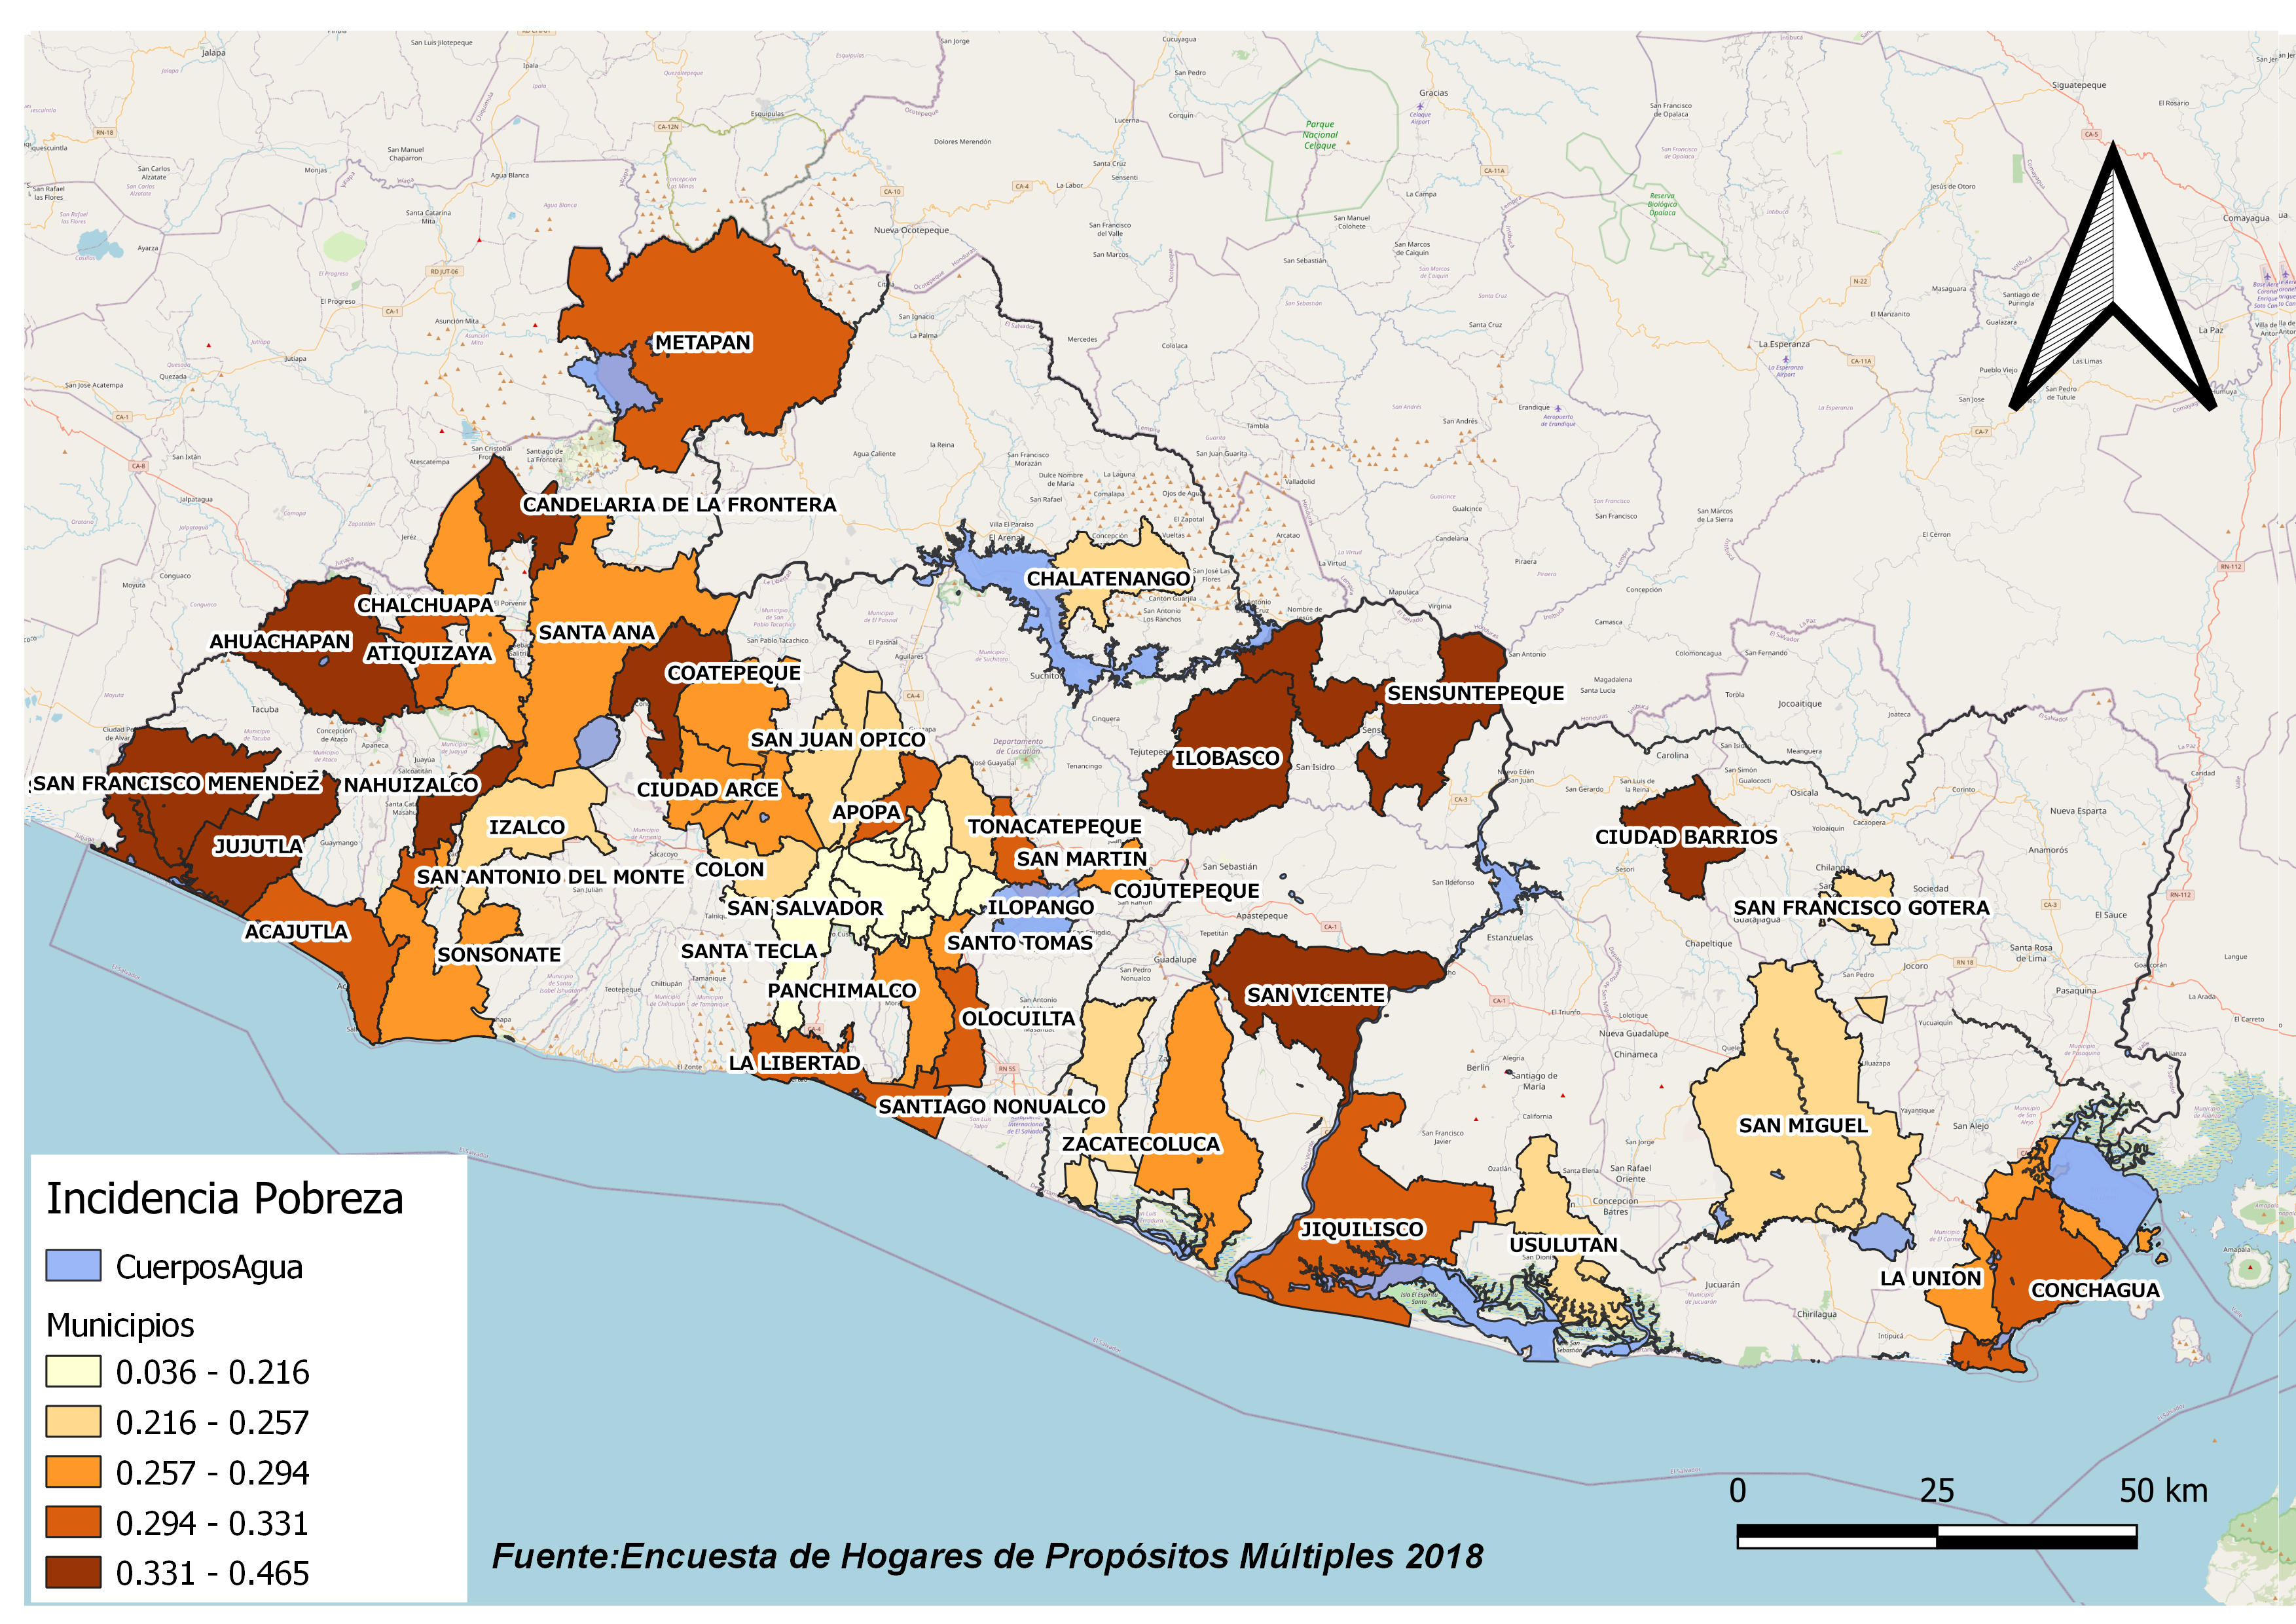
\includegraphics[width=1\linewidth]{Imagenes/Incidencia2}
	\caption{\textbf{\textit{Mapa de El Salvador por Municipios según Incidencia de Pobreza Proyectada.}} {\small El mapa de calor muestra los rangos por incidencia de pobreza calculado por medio de los índices FGT, a nivel proyectado para los 50 municipios autorepresentados de la EHPM 2018.}
	} 
	\label{fig:16}
	\resizebox{20 cm}{!} { }
	
\end{figure}


Usulután (Usulután) crece en un $19.1 \textperthousand$, es decir que su pobreza se traslada de $20.3 \textperthousand$ a $24.3 \textperthousand$,en la zona Occidental Metapán (Santa Ana) pasa de $25.7 \textperthousand$ de pobreza a $30.6 \textperthousand$ un crecimiento de $18.74 \textperthousand$, La Unión (La Unión) creció en $16.9 \textperthousand$ indicando que se traslada de $24.2 \textperthousand$ a $28.3 \textperthousand$ de hogares en pobreza, en séptima ubicación Izalco (Sonsonate), existe un crecimiento de $15.8 \textperthousand$ lo que indica que avanza de $22.1 \textperthousand$ a $25.6 \textperthousand$; el municipio de Sensuntepeque (Cabañas), crece su pobreza en $15.2 \textperthousand$, pasando de $33.0 \textperthousand$ a $38.0 \textperthousand$, La Libertad (La Libertad) la pobreza en sus hogares se desplaza de $28.5 \textperthousand$ a $32.6 \textperthousand$ indicando un crecimiento de $14.5 \textperthousand$, finalmente el municipio de Jiquilisco (Usulután), presenta en esos 10 primeros municipios que su condición de pobreza registrará un aumento en $14.7 \textperthousand$, indicando que pasará de $28.8 \textperthousand$ a $32.9 \textperthousand$, esta información se muestra para el resto de municipios y con mayor detalle en la tabla No. \eqref{Tabla 7} y a continuación la incidencia de pobreza que resultará con la perdida o disminución de las remesas se puede observar en el mapa contenido en el la Figura No. \eqref{fig:16}. Tal como se observa en la tabla y mapa la condición de pobreza aumentaría, es decir su incidencia y que las zonas más afectadas en ese clúster de 50 municipios, serán la occidental y la paracentral según se logra observar de forma general, los índices FGT muestran crecimiento, a donde se encuentra la brecha de pobreza se ve a continuación en el mapa de las brechas según la Figura No. \eqref{fig:17}:

\begin{figure}[H]
	\centering
	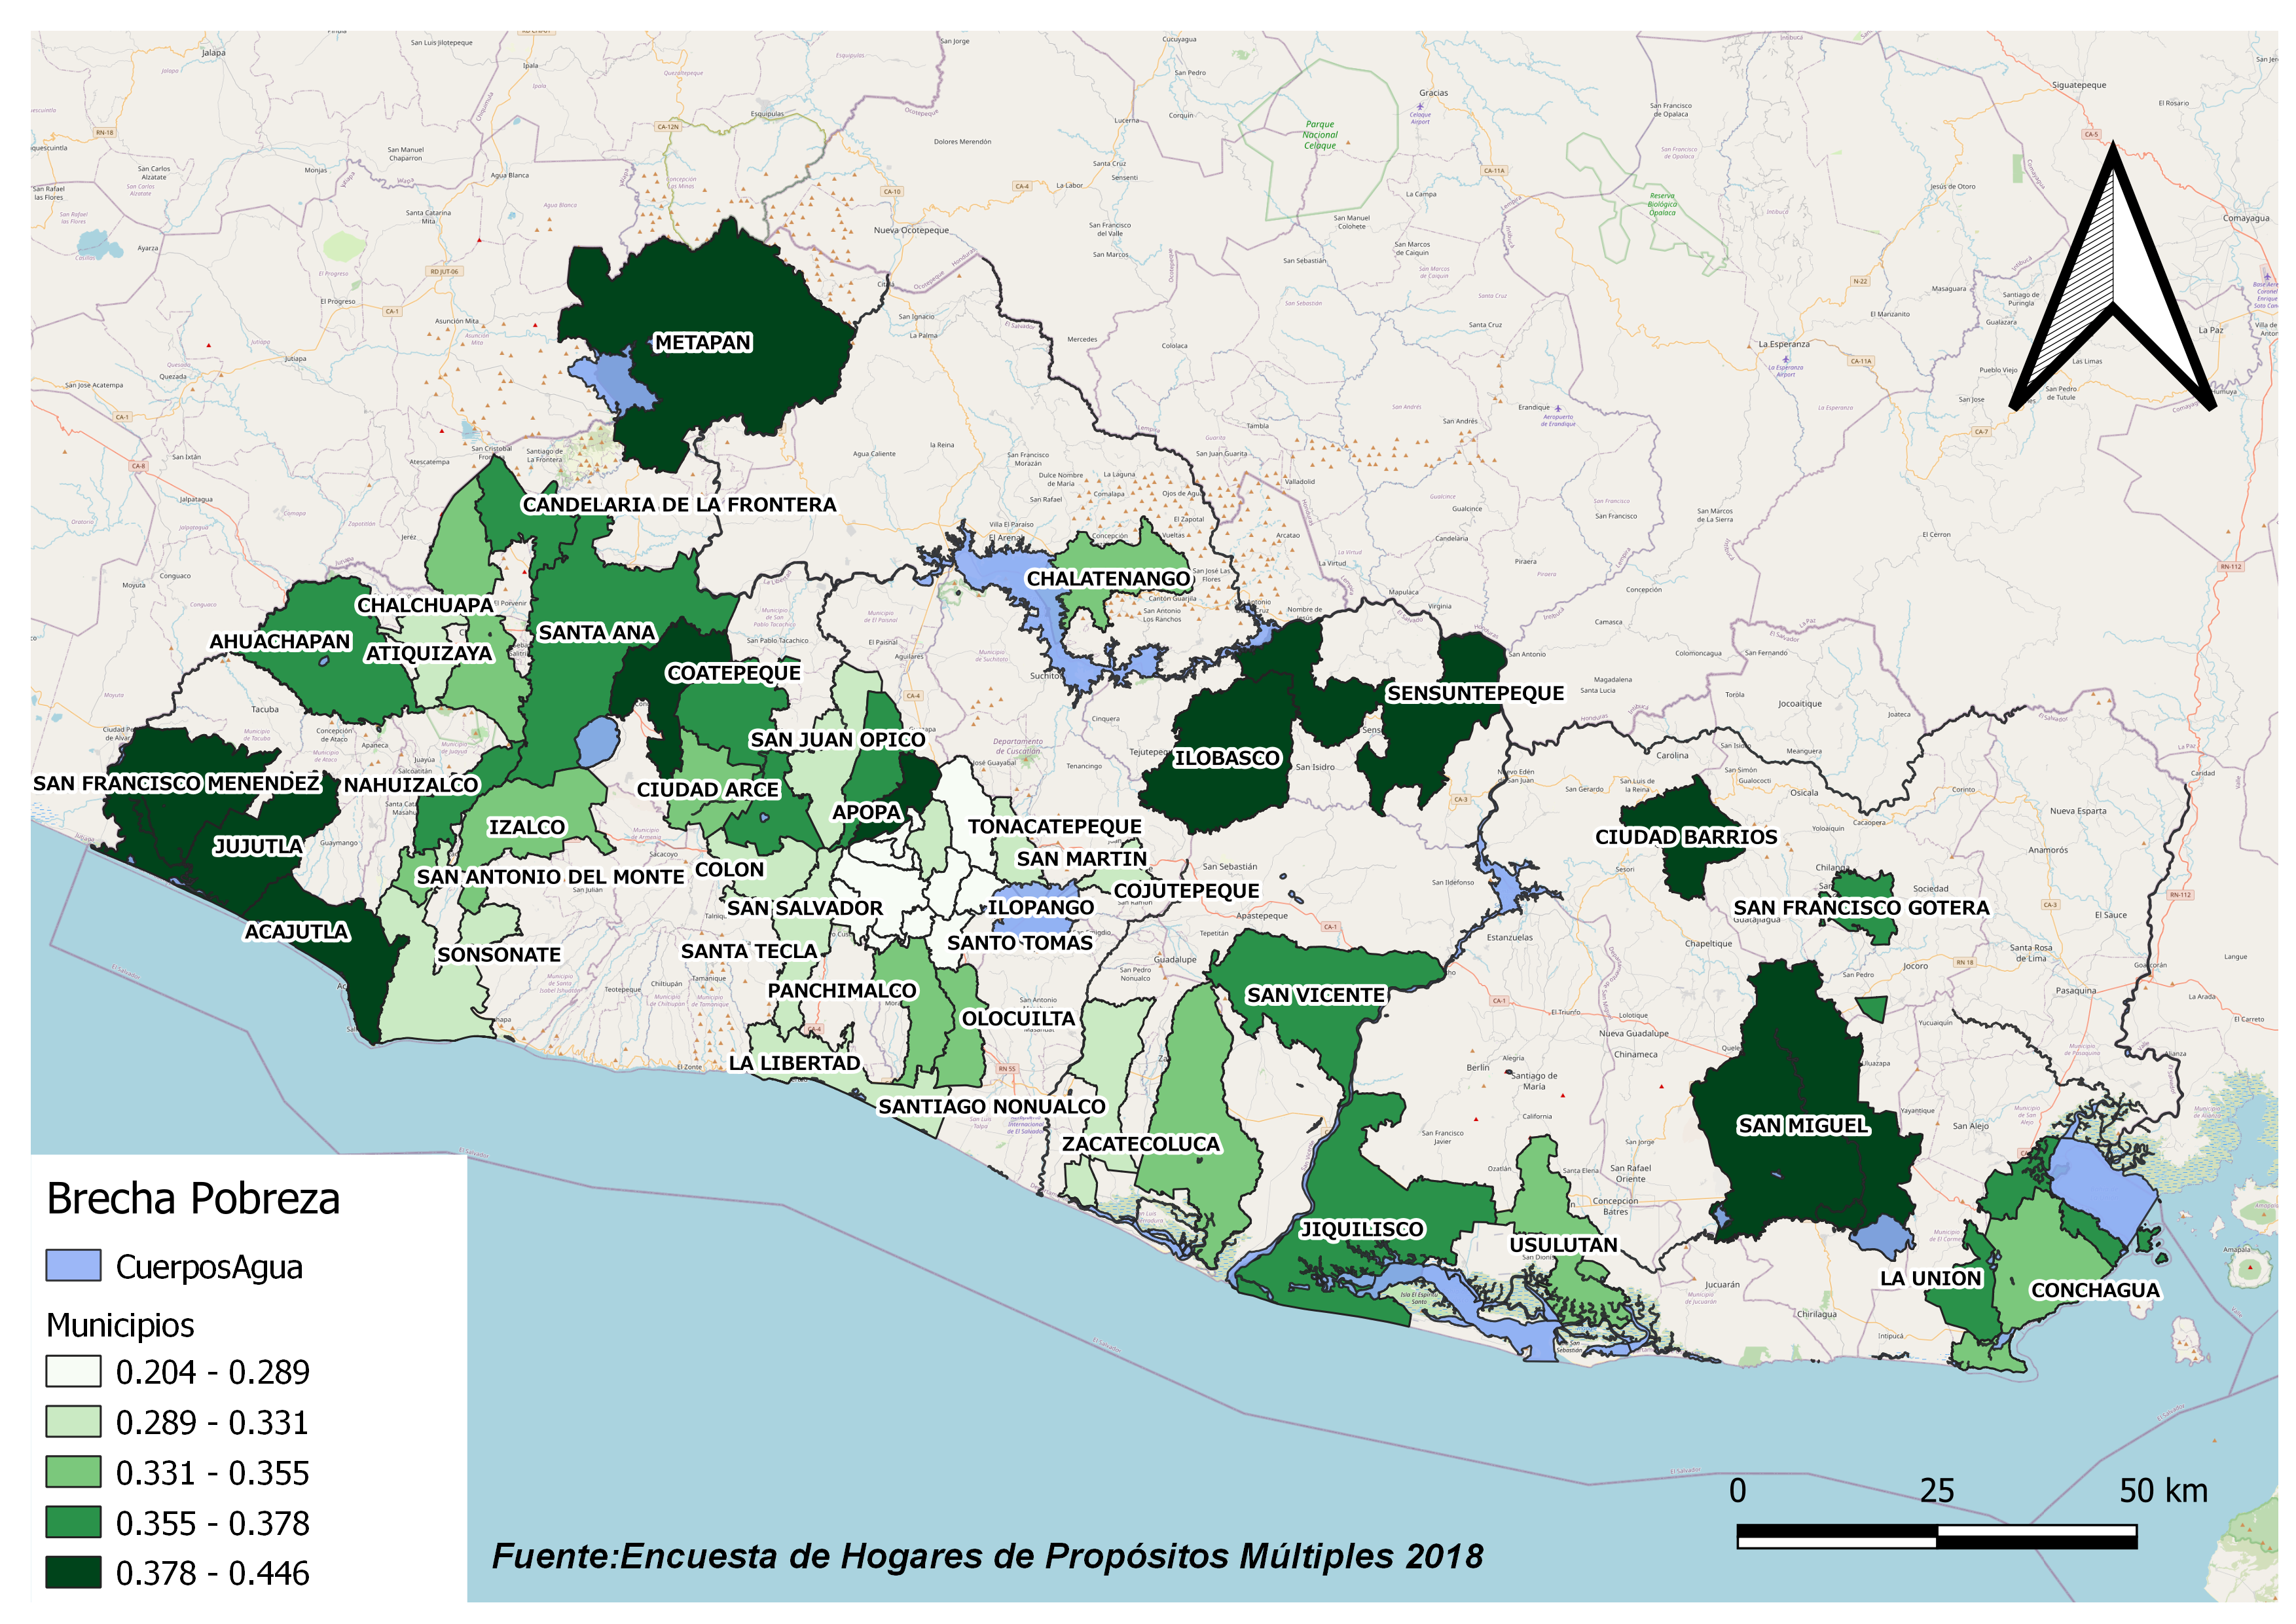
\includegraphics[width=1\linewidth]{Imagenes/Brecha2}
	\caption{\textbf{\textit{Mapa de El Salvador por Municipios según Brecha de Pobreza Proyectada.}} {\small El mapa de calor muestra los rangos por Brecha de pobreza calculado por medio de los índices FGT, a nivel proyectado para los 50 municipios autorepresentados de la EHPM 2018.}
	} 
	\label{fig:17}
	\resizebox{20 cm}{!} { }
	
\end{figure}

Como los indicadores son derivativos en cuanto a la brecha y severidad, se comportarán de forma similar, por ejemplo en la brecha de los primeros 5 municipios con mayores dificultades, son similares a los de severidad, recordando que en el proceso de su calculo, es el cuadrado de la brecha, el que representa la severidad, en el caso de la brecha esta representa la profundidad de la pobreza, por ejemplo los municipios que tendrían mayores repercusiones serían:  Ciudad Barrios (San Miguel), pasa de $41.9 \textperthousand$ a $44.6 \textperthousand$ con un crecimiento de $6.2 \textperthousand$, San Miguel (San Miguel), sus hogares en pobreza presentarán una brecha que crecerá de $6.1 \textperthousand$ lo que representa un traslado de $35.8 \textperthousand$ a $38.0 \textperthousand$, el municipio de Cuscatancingo (San Salvador) su pobreza se mueve de $24.7 \textperthousand$ a $26.2 \textperthousand$, lo que indica un crecimiento de $5.9 \textperthousand$, otro municipio que se verá afectado es San Martín (San Martín), cuya pobreza pasará de $29.9 \textperthousand$ a $31.6 \textperthousand$ un crecimiento de $5.6 \textperthousand$, finalmente Metapán (Santa Ana) su brecha aumentará de $5.4 \textperthousand$, a donde la brecha pasará de $36.2 \textperthousand$ a $38.2 \textperthousand$, según el mapa contenido en la figura No. \eqref{fig:17}. \\
  

%-----------------------------------------------

\section{DISCUSIÓN}
  
La discusión pone sobre el debate aspectos importantes de resaltar, posterior a la revisión de los datos; el primer componente es que la Economía de EE.UU. viene mostrando ya una caída en su crecimiento económico para el Trimestre 1, en $1.2 \textperthousand$ pero ya los especialistas pronostican una de las más profundas recesiones de la historia, incluso por arriba de la marcada en el año de 1930, incluso las proyecciones realizadas por organismos internacionales fueron o han sido muy optimistas con las tasas de crecimiento mundiales y de las estimaciones para las principales regiones económicas del planeta a causa del Covid-19.\\


Todas las medidas para recuperar la economía consisten en la emitir US$\$$700 trillones de dólares \footnote{\href{https://www.lavanguardia.com/economia/20200331/48144124018/coronavirus-crisis-medidas-estados-unidos-eurozona-bolsa.html}{https://www.lavanguardia.com/economia/20200331/48144124018/coronavirus-crisis-medidas-estados-unidos-eurozona-bolsa.html}}  dicha emisión a cargo de la Reserva Federal en los EE.UU. combinadas con políticas expansivas que tienen que ver con la compra de bonos del tesoro e hipotecarios, incluso la consideración de la compra de bonos basura y a nivel del Gobierno Federal ejecutar por aprobación del congreso, un gigantesco paquete de estímulos fiscales más del doble del paquete implementado en la crisis del 2009, dicho paquete incluye billonarias exenciones tributarias para las empresas, subvenciones a los oligopolios multinacionales del país y el envío de cheques por 1,200 dólares a más de cien millones de ciudadanos.\\
 

Estas medidas se suman a los $300,000$ millones de dólares en créditos puente a interés cero para empresas con problemas, a pesar de todas estas medidas para salvar la economía Estadounidense, hay especialistas de la misma FED, como Julian Kozlowski, Laura Veldkamp y Venky Venkateswaran que en su paper escrito en abril del presente año estiman tres escenarios no muy halagüeños por medio de un modelo econométrico para EE.UU./\footnote{\href{https://s3.amazonaws.com/real.stlouisfed.org/wp/2020/2020-009.pdf}{https://s3.amazonaws.com/real.stlouisfed.org/wp/2020/2020-009.pdf}}, y estos escenario revelan perdidas y caídas en el PIB de EE.UU. por $-18 \textperthousand$ 0 $-19 \textperthousand$ , ante la salida de capitales valoradas en un nivel de hasta el $-28 \textperthousand$ a largo plazo o fuertes pérdidas bancarias, implicando también bajas significativas para el empleo, capital, inversión y tasa de riesgo .\\

La expansión de la crisis económica de USA tendrá un desarrollo más fuerte para el segundo trimestre, un segundo componente que deriva de la recesión es el impacto en el empleo, debido al crecimiento de contagio que presentó el Covid-19 estados de la nación americana se reportaron rápidamente con cierres o lockdown a consecuencia de que la curva seguía su tendencia al alza, estas medidas repercutieron fuertemente en estados como: California, Texas, Florida, New York, Arizona, Illinois y New Jersey, dichos estado concentran el $71,2 \textperthousand$ de comunidad latina, aproximadamente unos $42.5$ millones de residentes de origen latino o hispano.\\

Sumado al componente de cierres por contagios del Covid-19, en varios estados se asocia inmediatamente el golpe en el mercado laboral, el cual ya reportaba para abril una cifra récord de $14,7 \textperthousand$, afectando a los sectores económicos de mayor importancia como lo son Ocio y hospitalidad relacionado al turismo y hostelería, Otros servicios, Comercio mayorista y minorista, Construcción, Agricultura, silvicultura, pesca y caza, Productos duraderos, Transporte y utilidades, Industria, Información, Servicios de educación y salud, Minería,canteras y extracción de petróleo y gas, entre otros sectores importantes para la nación americana y en donde los latinos tienen una principal participación, por ejemplo el sector de Ocio y hospitalidad, proporciona trabajo a más de 14.6 millones de personas de esa cifra el $24,0 \textperthousand$ lo integra empleo latino, es decir aproximadamente unos 3.5 millones, pero dicho sector registra la mayor perdidas de empleo con una tasa de $39,3 \textperthousand$ al mes de abril, un nivel muy significativo de desempleados.\\

Lógicamente con las anteriores cifras, el desempleo tocó principalmente a los latinos, en vista que esta reportó para el mismo mes de abril el $18,9 \textperthousand$ trayendo consigo la proyección que existirá una reducción de las remesas o transferencias desde los EE.UU., se estima que del total de 59 millones de latinos un $9.3 \textperthousand$ son centroamericanos, por ende el impacto en las remesas se espera muy signifcativo, de hecho el Banco Mundial estima una caída por US$\$$445,000 millones \footnote{\href{https://www.bancomundial.org/es/news/press-release/2020/04/22/world-bank-predicts-sharpest-decline-of-remittances-in-recent-history}{https://www.bancomundial.org/es/news/press-release/2020/04/22/world-bank-predicts-sharpest-decline-of-remittances-in-recent-history}} lo que representaría un $19.7 \textperthousand$, según se citan las palabras del presidente del Banco: “Las remesas son una fuente de ingresos vital para los países en desarrollo. La recesión económica actual provocada por la COVID-19 está afectando gravemente la capacidad de enviar dinero a los hogares de origen y por eso es aún más urgente que acortemos el tiempo que llevará la recuperación para las economías avanzadas”, sostuvo David Malpass, presidente del Grupo Banco Mundial. ”Las remesas ayudan a las familias a costear alimentos, atención de la salud y otras necesidades básicas.\\

De hecho con la construcción del sencillo modelo de estimación de monto de remesas trimestrales explicado por el monto del PIB real de los EE.UU. de forma trimestral, afectado por una contracción económica del $18.0 \textperthousand$, repercute según el pronóstico del modelo en una perdida por US$\$$ 467.32 millones para el segundo trimestre, indicando una reducción considerable, en vista de que pasa de un monto de US$\$$ 1,313.45 millones para el Primer trimestre 2020 a un monto por US$\$$ 846.13 millones, esto equivale a una descenso por $35.6 \textperthousand$ muy por arriba del pronostico que plantea el Banco Mundial de casí un $19.7 \textperthousand$, explicado por las altas tasas de desempleo en sectores estratégicos de la economía estadounidense a donde se emplean a muchos compatriotas latinos.\\
    
Con dichas perdidas en los montos de las transferencias monetarias directas, la pobreza fue recalculada para El Salvador en un escenario cuya recomposición se construyo con una baja del $35.6 \textperthousand$ del ingreso por remesas que utiliza la EHPM 2018 y que al ser estimada para los ingresos familiares y luego percapitados y comparados a las CBA tanto urbana como rural, la pobreza crece de un $26.2 \textperthousand$ a un $28.5 \textperthousand$, pero que significado tiene este aumento en 2.3 puntos en la pobreza, el significado es preocupante, debido a que solo se esta cuantificando el impacto por reducción por remesas sin adicionar el impacto o escenario que tendrá la contracción de la economía nacional o la perdida interna del mercado laboral a causa de las medidas de confinamiento; el aumento de la pobreza muestra que $42,924$ hogares o $142,358$ personas pasaran a ser pobres, o viéndolo desde la perspectiva contraria, podemos decir que  $142,358$ personas cuyas condiciones no eran de pobreza pasarán a engrosar la capa de pobreza relativa o extrema con la disminución en los montos por remesas debido a una contracción económica en los EE.UU., esto signifcaría un traslado del universo de 2.05 millones a  2.19 millones de personas en pobreza. \\

Los resultados en la recomposición de la pobreza indican que los indices de pobreza FGT medidos para los 50 municipios autorepresentados, se veran incrementados por ejemplo la incidencia y profundidad de la pobreza o conocida también como brecha de pobreza se focaliza en las regiones occidentales y paracentrales y municipios como San Miguel, San Salvador y Conchagua presentarán aumentos en la cantidad de hogares que pasarán a ser pobres, pero en cuanto a la profundidad o alejamiento de los ingresos para cubrir una CBA serán los municipios de Ciudad Barrios, San Miguel, Cuscatancingo y San Martín serán los principalmente impactados en similar proporción con su condición de severidad de la pobreza. Esto se suma a los problemas de seguridad alimentaria que estima el Programa Mundial de Alimentos PMA en donde destaca que en el país se encuentran 239,000 personas en fase de crisis alimentaria y 63,000 en emergencia, según su informe global sobre crisis alimentaria 2020\footnote{\href{https://www.wfp.org/publications/2020-global-report-food-crises}{https://www.wfp.org/publications/2020-global-report-food-crises}} 

%---------------------  
\newpage
\section{CONCLUSIONES}

\begin{itemize}
	\item Se concluye en similar perspectiva a la CEPAL \cite{cepal2020dimensionar}, que indica que la crisis del Covid-19 no solo se ha convertido en una crisis de salud pública, sino también ya se convierte en una crisis económica y social que requiere todo el esfuerzo máximo de los gobiernos para resolverlas.
	\item El impacto del Covid-19 en la economía de los EE.UU. es inminente y este escenario podría agravar las condiciones de empleo de la población latina, en vista que se han afectado en gran medida Estados donde residen una buena cantidad de comunidad latina o hispana, como California, Texas y Florida por mencionar algunos.
	\item Se concluye además que el desempleo latino reportado en un $18,9 \textperthousand$, se verá incrementado para lo que resta del año, producto de que la expansión en la recesión económica de los EE.UU. según especialista tenderá a profundizarse a escenarios de mayores caídas del PIB real, incluso a niveles de $-19.0 \textperthousand$. 
	\item Los principales sectores económicos de EE.UU. a donde se emplea mucha comunidad latina o hispana, se han visto mayormente afectados con una serie de contagios del virus, dando pie a muchos cierres obligados, lo que derivó en altas tasas de desempleo, planteando con ello, através del modelo una extrapolación que indica una reducción significativa del $35.6 \textperthousand$ en las remesas nacionales para el segundo trimestre.
	\item Se estima que la reducción en las remesas incrementará la pobreza en $28.5 \textperthousand$, en otras palabras enviará a $142,358$ personas que no eran pobres a sumarse a las capas de marginidad y exclusión, es decir, que estas personas presentaran serios problemas o dificultades en sus ingresos para poder conseguir la cobertura del costo de una canasta básica alimentaria CBA.
	\item Los cálculos de los indicadores FGT concluyen que existirá un incremento en la incidencia en la pobreza y que se presentará un cambio en la profundidad y severidad de la pobreza, afectando en mayor medida a las regiones ya vulnerables como lo son la región occidental y paracentral en el marco de los 50 municipios autorepresentados que define la EHPM 2018.
	\item La profundización o incrementos en las condiciones de los niveles de pobreza, conlleva el monitoreo de la seguridad alimentaria, este problema se suma o entrelaza a los más de 302 mil individuos que venían ya presentando fase de crisis y urgencia alimentaria desde el año 2019 según el reporte global del PMA, por esos motivos se observan muchas banderas blancas a nivel nacional y que el Gobierno pretende cubrir con la entrega de una canasta básica de alimentos. 
	\item El Universo de pobreza que actualmente representa a 491,323 hogares pasará a 534,247 o lo que indica un poco más de 2.1 millones de personas en condiciones precarias, esto obligará al Estado a constituir un Plan o Programa de Emergencia Económica o Social que cubra el deficits de ingresos por perdida de remesas para impedir que la pobreza aumente, esto necesitará en estimaciones gruesas un fondeo de aproximadamente US$\$$342 millones, para otorgar un monto de una canasta básica alimentaria de US$\$$107 durante 6 meses, aclarando que esto es solo sirve para cubrir la pobreza derivada solo por disminución por remesas no incluye los efectos por perdida de las condiciones de empleo interno.
\end{itemize}


%---------------------  
\newpage
\section{RECOMENDACIONES}


\begin{itemize}
	\item Se recomienda crear un observatorio nacional que monitoree desde una perspectiva multidisciplinaria el seguimiento y el impacto del Covid-19 en el país, aportando además un enfoque multidimensional de salubridad, una dimensión económica y una dimensión social, con la finalidad de que proporcione información técnica científica para el respaldo de las decisiones en política nacional para el manejo de la pandemia, recordando que el Covid-19 ha venido para quedarse según lo manifiestan algunos expertos en salud y habrá que adaptarse para sobrellevar una nueva normalidad.
	\item Será importante conformar en la dimensión social un programa o plan de alivio a la pobreza, en vista que las consecuencias de la recesión económica que se acerca, traerá grandes impactos en las condiciones de pobreza, y será necesario detener su profundización, el análisis estima un fondeo de aproximadamente US$\$$342 millones para 6 meses, solo para solventar la reducción de los montos por remesas no incluye el impacto global por perdida de empleo interno en el mercado laboral como producto del confinamiento, no incluye las otras relaciones o efectos económicos derivados de esa fuerte contracción que sufrirá EE.UU. en su economía, como por ejemplo comercio exterior, endeudamiento, medidas migratorias, mercado financiero, etc..
	\item Sumado al programa de alivio a la pobreza, se debe de crear un componente que apoye la resiliencia contra el hambre, que se puede convertir en un problema crónico o profundo que acompaña a la pobreza, dado el PMA proyecta a 302 mil personas en fase crítica y urgente, pero esta cifra puede escalar a niveles más altos durante el periodo de post-pandemia.
	\item El aumento de hogares en las franjas de pobreza tal como lo plantea la Cepal  en su informe \cite{cepal2020desafio}, puede propiciar el riesgo del aumento del trabajo infantil y una mayor deserción escolar porque los hogares priorizarán el ingreso para obtener alimentos durante la crisis.
	\item En esta situación de extremo golpe al ingreso y a la economía, incluso hay que valorar traer al debate y análisis la pertinencia de contar nuevamente con una política monetaria que complemente la política fiscal del Estado y tener más herramientas efectivas que contrarresten las consecuencias de impacto económico que se avecina, barajar un bimonetarismo real o una desdolarización debe ser parte del contenido del debate o la acción en la política económica a ejecutar.	
	\item Se recomienda desarrollar y complementar la investigación para medir el impacto en la pobreza derivada de la perdida de los empleos como producto de las medidas de confinamiento y la recesión económica.
	\item La ayuda estatal debe de priorizar los municipios más pobres del país, los 50 municipios autorepresentados que define la EHPM puede servir de referencia, aunque será importante explorar otras fuentes de información. 
	\item Finalmente se recomienda tomar la propuesta de la Cepal, de valorar establecer una renta básica universal para poder cubrir los efectos económicos del Covid-19 y detener la expansión de los niveles de pobreza, más otras medidas estructurales y de análisis al modelo económico vigente que conlleven a construir ese marco de reformas que traigan efectivamente mayor desarrollo, bajo otra óptica diferente a la tradicional.

\end{itemize}

